% Luigi: immagini pdf 
% Luigi: paper cubi / quadrati
% Luigi: preparazione campioni

\documentclass{article}
\author{Alessio Cimma, Andrea Giura, Luigi Ribotta}
\title{Tip reconstruction with automatic shape recognition}

\usepackage{graphicx}               
\usepackage{booktabs}
\usepackage{caption}
\usepackage{amsmath}
\usepackage{tikz}
\usepackage{listings}

\definecolor{backcolor}{rgb}{0.95, 0.95, 0.95}
\definecolor{codegreen}{rgb}{0.25, 0.45, 0.25}

% Define Python style
\lstdefinestyle{Pythonstyle}{
    language=Python,
	basicstyle=\scriptsize\ttfamily,
	tabsize=4,
    backgroundcolor=\color{backcolor},
    commentstyle=\color{codegreen},
    keywordstyle=\color{magenta},
    identifierstyle=\color{violet},
    stringstyle=\color{green!50!black},
    showstringspaces=false,
	showtabs=false,
    numbers=left,
    numberstyle=\tiny,
    numbersep=5pt,
    breaklines=true,
    extendedchars=true,
    linewidth=\textwidth,
	morekeywords={*,...}
}

\begin{document}

\maketitle

\newpage
\tableofcontents
\newpage


\begin{abstract}
    In this technical report, we will dive into the explanation of the working principle behind the code we'll be using to generate processed convoluted AFM images. The main idea behind this project relies on the generation of ideal structures and using them as a kernel for a convolution (an erosion to get the tip and a dilation to get the deconvoluted image). Using a raytracer technique we will simulate an ideal monoatomic tip that scans our ideal sample resulting in an ideal AFM topography. When combaining this information with the original AFM data and we get through all the passages explained in Villarubbia's work [4], we can finally obtain our final result.
    
    The new added feature fast and reliable generation of this ideal sample, since in previous works [3] there was a more individual approach to a single type of nanostructure based on specific math formulas. Now it is possible to generate multiple models of the expected size and orientation, and analizing them using a image recognition algorithm, speeding up many times the whole process.
    \\[1cm]
    In questo rapporto tecnico, affronteremo la spiegazione del principio di funzionamento che si trova alla base del codice usato per la generazione di immagine convolute partendo da immagini AFM. L'idea generale dietro a questo progetto si basa sulla generazione di strutture ideale che andremo ad utilizzare come kernel per una convoluzione (un'erosione per la creazione della punta e una dilatazione per l'immagine deconvoluta). Usando la tecnica del raytracer, simuleremo una punta monoatomica ideale che andrà a scanerizzare il nostro campione ideale generando così una topografia AFM ideale. Quando combiniamo questa informazione con la topografia AFM originale e applicchiamo i vari passaggi descritti nel lavoro di Villarrubia [4], possiamo finalmente ottenere il risultato finale.
    
    La novità aggiunta in questo lavoro si basa sulla generazione del campione ideale in maniera molto più rapida e precisa, nonchè estremamente versatile. In lavori precedenti [3], si tendeva a trovare un approccio che fosse estremamente preciso, ma funzionale solo per un determinato tipo di nanoparticella, basata su determinate funzioni matematiche. Ora invece è possibile creare e gestire molteplici modelli (di forme, orientamenti e dimensioni date) e analizzarle usando un algoritmo di riconoscimento immagini, velocizzando complessivamente di molto tutto questo processo. 
    
\end{abstract}

\newpage
\section{Introduction}\label{sec:Introduction}

Atomic Force Microscopy (AFM) stands as one of the foremost tools in the field of nanotechnology, offering unparalleled precision in imaging and manipulation at the atomic scale. 

The AFM microscope operates on the principle of scanning a sharp tip across the surface of a sample, detecting interactions between the tip and the sample to generate high-resolution images. Through the interaction of many forces, including van der Waals, electrostatic, and magnetic interactions, the tip can precisely map the surface topography with nanometer-scale resolution. Such precision has led to its widespread adoption across various scientific disciplines, from materials science to biology [1, 2, 3].

Integral to the functionality of the AFM microscope is the concept of tip reconstruction, a process aimed at ensuring the accuracy and reliability of imaging results. The history of AFM tip reconstruction traces back to the early days of AFM development, when Villarubbia in his paper [4] introduced the concept of the tip reconstruction.

In particular we will be focusing on the aspect and working principle of a morphological filter, which is an approach to remove the interference generated by the physical presence of the tip during the measurement. The process consists in extrapolating the tip shape from the image knowing in advance some parameters of the sample we are going to study. We will be finally using the reconstructed tip to deconvolute the image and obtain the final image, which will have a far better spatial resolution. 

In tandem with advancements in AFM tip reconstruction, parallel progress has been made in the field of raytracing techniques used in computer graphics. One of the critical components in raytracing is the z-buffer, a fundamental data structure employed to resolve visibility and generate accurate meshes. The fusion of AFM data with raytracing techniques represents a paradigm shift in the field of nanostructure generation. This approach enables the creation of precise nanostructures that serve as ideal templates for erosion tip reconstruction algorithms.

\newpage

\section{Structure generation}\label{sec:Structure_generation}

The general method used to create different structures is based on the generation of meshes made of triangles using some known parameters. These meshes can then be rendered using a technique called z-test (also known as depth-test) which relies on testing the distance at which a certain point is from the camera. If another point that should be drawn in the same pixel results to be closer, it will sostitute the previous one. This will ensure a correct occlusion handling.
\\[.5cm]
Since we need to recreate the tip shape, we need to firstly generate an ideal image, that can be thought as the image generated by an ideal point-shaped tip. Approximated to a monoatomic tip, resembling a Dirac's delta. If we simulate what a ray of light does as it exits the camera and tries to reach the sample, we can calculate how far is the sample (height information) and what part of the sample it hit (morphological information). We also want to correlate the tip reconstruction with working principle of a raytracers, beacuse of the big steps that were made in the recent years in this field, enabling us to easily update the work of this paper to a real-time application.
\\[.5cm]
Raytracers are also used in the simulation of optical and electronic microscopes, since the behaviour on which this system are based is equal. We want to use this approach on an AFM, so it makes sense to simulate an ideal tip of the smallest size possible.
\\[.5cm]
Raytracers use this approach to simulate and correctly identify which triangle a ray has hit and understanding what the resulting pixel color will be. 
\\[.5cm]
Raytracers usually will do some other shader calculation in order to create photo-realistic images, but for this project, we will borrow just the algorithm for correctly rendering triangles and their occlusions.
\\[.5cm]
Since this technique is identical to a pipeline used in real-time applications called rasterization and fragment processing (which is quicker) we will be focusing on this approach instead.
\\[.5cm]
We can then create a standard and normalized model of each structure we want to study (spheres, cubes, steps, ecc.) and given an external input of parameters generate the model of the correct size, orientation and position using scale, rotation and traslation.
\\[.5cm]
This way we generate an array of triangles that then will be rendered resulting in the ideal structure we needed.

\newpage

\subsection{Triangles}\label{subsec:Triangles}

We can divide the pipeline in 3 sections:

\begin{itemize}
    \item Mesh generation
    \item Rasterization
    \item Fragment processing 
\end{itemize}

\subsubsection{Mesh generation}

The single models will be created in the corresponding functions, which will generate 2 arrays of data (position of vertices and links to unite the vertices) starting from the base model obtained through an \texttt{*.obj} files. Using the different matrices for scale, rotation and translation we can position it how and where we want. 
\\[.5cm]
The model will always be generated with a bounding box that stratches from $P_{min}(-1,-1,-1)$ to $P_{max}(1,1,1)$, so to generate the disered model we will apply in order:

\begin{itemize}
    \item Rotation along the z-axis (the model will always mantain the same base, just different orientation):
    $$R = \begin{pmatrix} \cos(\alpha) & \sin(\alpha) & 0 & 0 \\ -\sin(\alpha) & \cos(\alpha) & 0 & 0 \\ 0 & 0 & 1 & 0 \\ 0 & 0 & 0 & 1 \end{pmatrix}$$

    \item Scaling and traslation along x,y,z-axis (the grounding of the model is handled differently in each function): 
    $$R = \begin{pmatrix} S_x & 0 & 0 & 0 \\ 0 & S_y & 0 & 0 \\ 0 & 0 & S_z & 0 \\ T_x & T_y & T_z & 1 \end{pmatrix}$$

\end{itemize}

\subsubsection{Rasterization}
Please pay attention that this process is applied to each triangle in the triangle buffer
\\[.5cm]
Rasterization is the process that we can use to determine which pixels are inside a triangle and which are not. It is based on the barycentric coordinates. These are some values that represent a point within a triangle as a weighted sum of its vertices. Which means that if a point inside a triangle, then it needs to satisfy the equation:
$$w_1 + w_2 + w_3 = 1$$ and most importantly, each one of this weights must be in the interval between $(0, 1)$
\\[.5cm]
In the implementation there's also a change of the coordinates system, which increases performance by not testing a bunch of pixels that are known to not be part of the triangle. This is done by testing pixels moving along scanlines that are aligned with one of the edges of the triangle.
\\[.5cm]
\paragraph{Artifacts:} A known issue is that the float to integer approximation that is used to transform coordinates in array indices may generate some blank spots as reported in Figure \ref{fig:artifacts} (a).
This artifact is solved using a bias vector, which adds to each point $0.5$ pixel. It doesn't change the final output, but it helps to create more consistent data as reported in Figure \ref{fig:artifacts} (b).
\begin{center}
    \begin{minipage}{0.45\textwidth}
        \includegraphics*[width=\linewidth]{../images/artifact_ON.png}
    \end{minipage}
    \hfill
    \begin{minipage}{0.45\textwidth}
        \includegraphics*[width=\linewidth]{../images/artifact_OFF.png}
    \end{minipage}
    \label{fig:artifacts}
    \captionof{figure}{Fixing artifacts: a) Before bias application, b) After bias application}
\end{center}

\subsubsection{Fragment processing}
Using the barycentric coordinates we can obtain for free a linear interpolation of each point in correlation with the vertices. This means that each property that the vertices have in common can be interpolated. Some examples might be:
\begin{itemize}
    \item position
    \item color
    \item depth
    \item normal
    \item UV mapping
\end{itemize}
This means that knowing the position of the vertices can lead us knowing at which depth / height they are in our scene.

\begin{figure}[h]
    \centering
    \begin{tikzpicture}
        % Sample at the bottom
        \draw (0,0) -- (3,0);
        \draw (3,0) -- (3,1.5);
        \draw (3,1.5) -- (5,1.5);
        \draw (5,1.5) -- (5,0);
        \draw (5,0) -- (10,0);
        \draw (7,1.5) node {Rough Sample};
        
        % Camera on top
        \draw (4.5,7) -- (3.8,5);
        \draw (4.5,7) -- (5.2,5);
        \draw (3.8,5) -- (5.2,5);

        \draw (6,6) node {Camera};
        \draw (10,.2) node {h = 0};
        \draw (10.5,7) node {h = Camera.Z};
        
        % Tract line
        \draw[->,thick] (4.5,7) -- (4.5,1.5);
        \draw[dashed,thick] (8.75,7) -- (8.75,0);
    \end{tikzpicture}
    \caption{Rough sample viewed by camera. The Z coordinate corresponds to the height of the sample (assuming ground level = 0)}
\end{figure}

\begin{center}
    \begin{minipage}{0.45\textwidth}
        \includegraphics*[width=\linewidth]{../images/depth_test.png}
    \end{minipage}
    \hfill
    \begin{minipage}{0.45\textwidth}
        \includegraphics*[width=\linewidth]{../images/bary_test.png}
    \end{minipage}
    \captionof{figure}{Example of interpolation based on: a) depth test, b) barycentric coordinate}
\end{center}

\paragraph{Linear interpolation equation:} Given the 3 vertices $P_i(x,y,z)$ and optionally another attribute, we can use the $x$ and $y$ coordinates to interpolate these values as follows:
$$A_p = A_1u_1 + A_2u_2 + A_3u_3$$
Specifically the weights can be computed as:
$$u_1 = \frac{(y_2 - y_3)(x_p - x_3) + (x_3 - x_2)(y_p - y_3)}{(x_1 - x_3)(y_2 - y_3) - (x_2 - x_3)(y_1 - y_3)} \\$$
$$u_2 = \frac{(y_3 - y_1)(x_p - x_3) + (x_1 - x_3)(y_p - y_3)}{(x_1 - x_3)(y_2 - y_3) - (x_2 - x_3)(y_1 - y_3)} \\$$
$$u_3 = 1 - u_2 - u_1$$
This is the explicit calculation that alternativly can be computed as the cross product of two edge vectors:
$$u_1 = (v_2 - v_3) \times (v_2 - p) \\$$
$$u_2 = (v_3 - v_1) \times (v_3 - p) \\$$
$$u_3 = (v_1 - v_2) \times (v_1 - p)$$

\newpage

\subsection{Spheres}\label{subsec:Spheres}

The model is created in Blender using an icosphere with 5 subdivisions. It is centered in the origin with radius $=1$.
The model is imported and scaled by a radius in \texttt{StructGenerator.sfera()}.
\\[.5cm]
In \texttt{MacroController.single\_sphere()} it is then translated by a vector $v = (x, y, z)$ to it's new position. The z equals to $r/2$ to position the base of the sphere on the floor.

\begin{center}
    \begin{minipage}{0.3\textwidth}
        \includegraphics*[width=\linewidth]{../images/sfera_singola.png}
    \end{minipage}
    \hfill
    \begin{minipage}{0.3\textwidth}
        \includegraphics*[width=\linewidth]{../images/sfera_doppia.png}
    \end{minipage}
    \hfill
    \begin{minipage}{0.3\textwidth}
        \includegraphics*[width=\linewidth]{../images/sfera_statistica.png}
    \end{minipage}
    \captionof{figure}{Example of usage of spheres: a) Single b) Double c) Statistic}
\end{center}

\newpage

\subsection{Nanosheets}\label{subsec:Nanosheets}

The model is created in Blender using a cube divided in half along the $Z$ axis. It is centered in the origin with half size $=1$.
The model is imported and in \texttt{StructGenerator.nanosheet()} the following transformations are applied:
\begin{itemize}
    \item $Z$ scale (to unform the scale between the height and the width) the value equals to: $$S_Z = h / w$$
    \item $XY$ scale (to generate the inset of the top and bottom faces) the value equals to: $$S_{XY} = 1 - \frac{h_\text{eff}}{\tan(68.3^{\circ})}$$ where $h_\text{eff}$ is the new calculated height.
\end{itemize}
\begin{center}
    \includegraphics[width=.6\textwidth]{../images/transformations_nanosheet.png}
    \captionof{figure}{a) Original cube, b) $Z$ scale, c) $XY$ scale inset}
\end{center}
It is then:
\begin{itemize}
    \item Translated along the $Z$ axis to floor it 
    \item $XYZ$ scaled to match the desired size 
\end{itemize}
\begin{center}
    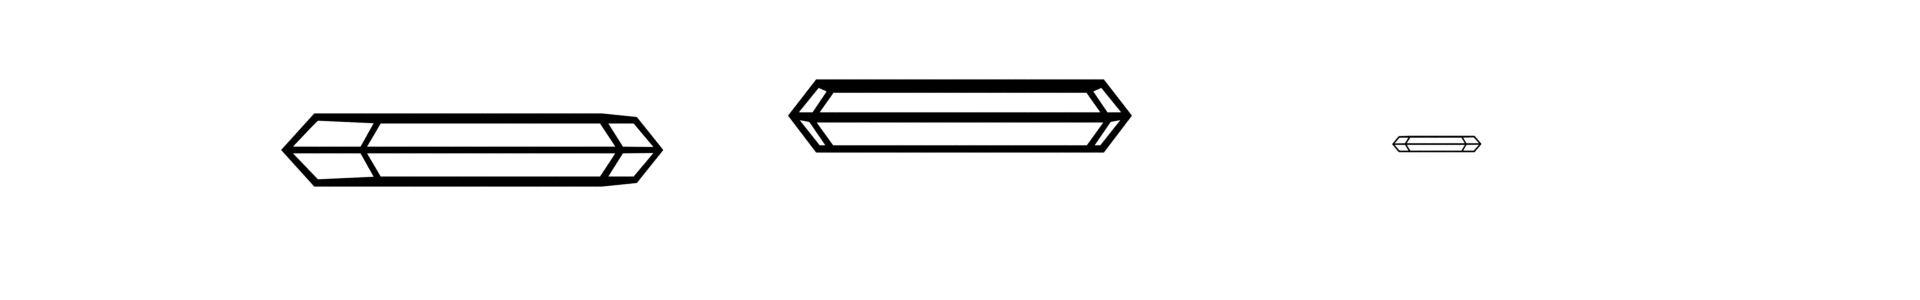
\includegraphics[width=1\textwidth]{../images/transformations2_nanosheet.png}
    \captionof{figure}{a) Original nanosheet, b) Floor process, c) $XYZ$ scaling size}
\end{center}
Until the last passage the model remains normalized (half size $=1$), this means that in order to match the desired size, we need to scale everything by a factor of $(\text{Nominal Size} / 2)$
\\[.5cm]
In \texttt{MacroController.single\_nanosheet()} it is then translated by a vector $v = (x, y, z)$ to it's new position. The z equals to $0$ to position the base of the nanosheet on the floor.

\begin{center}
    \begin{minipage}{0.3\textwidth}
        \includegraphics*[width=\linewidth]{../images/nanosheet_singola.png}
    \end{minipage}
    \hfill
    \begin{minipage}{0.3\textwidth}
        \includegraphics*[width=\linewidth]{../images/nanosheet_doppia.png}
    \end{minipage}
    \hfill
    \begin{minipage}{0.3\textwidth}
        \includegraphics*[width=\linewidth]{../images/nanosheet_statistica.png}
    \end{minipage}
    \captionof{figure}{Example of usage of nanosheets: a) Single b) Double c) Statistic}
\end{center}

\subsection{Bipiramids}\label{subsec:Bipiramids}

The model is created in Blender using a cube divided in half along the $Z$ axis. It is centered in the origin with half size $=1$.
The model is imported and in \texttt{StructGenerator.bipiramid()} the following transformations are applied:
\begin{itemize}
    \item $Z$ scale (to unform the scale between the height and the width) the value equals to: $$S_Z = h / w$$
    \item $XY$ scale (to generate the inset of the top and bottom faces) the value equals to: $$S_{XY} = 1 - \frac{h_\text{eff}}{\tan(68.3^{\circ})}$$ where $h_\text{eff}$ is the new calculated height.
\end{itemize}
\begin{center}
    \includegraphics[width=.6\textwidth]{../images/transformations_bipiramid.png}
    \captionof{figure}{a) Original cube, b) $Z$ scale, c) $XY$ scale inset}
\end{center}
After that it must be positioned onto one of the diagonal faces, since the small bottom base will not ensure the maximum equilibrium. This is done by moving along the $Z$ axis the model so that the bottom base sits on the floor. At this point a rotation matrix that rotates along the $X$ axis is applied with an angle of $68.3^{\circ}$
\begin{center}
    \includegraphics[width=.6\textwidth]{../images/transformations2_bipiramid.png}
    \captionof{figure}{Translation along $Z$ axis to floor the model and along the $Y$ axis to center the model with it's center of mass}
\end{center}
It is finally:
\begin{itemize}
    \item Translated along the $Z$ axis to floor it 
    \item Translatex along the $Y$ axis to center it on its center of mass
    \item $XYZ$ scaled to match the desired size 
\end{itemize}
Until the last passage the model remains normalized (half height $=1$), this means that in order to match the desired size, we need to scale everything by a factor of $(\text{Nominal Height} / 2)$
\\[.5cm]
In \texttt{MacroController.single\_bipiramid()} it is then translated by a vector $v = (x, y, z)$ to it's new position. The z equals to $0$ to position the base of the bipiramid on the floor.

\begin{center}
    \begin{minipage}{0.3\textwidth}
        \includegraphics*[width=\linewidth]{../images/bipiramid_singola.png}
    \end{minipage}
    \hfill
    \begin{minipage}{0.3\textwidth}
        \includegraphics*[width=\linewidth]{../images/bipiramid_doppia.png}
    \end{minipage}
    \hfill
    \begin{minipage}{0.3\textwidth}
        \includegraphics*[width=\linewidth]{../images/bipiramid_statistica.png}
    \end{minipage}
    \captionof{figure}{Example of usage of bipiramids: a) Single b) Double c) Statistic}
\end{center}

\newpage

\subsection{Steps}\label{subsec:Steps}

\subsubsection{Overview}\label{subsubsec:Step_overview}
In this chapter we will illustrate how it's possible to reconstruct the tip from an AFM image of the 3D steps. The process will consist in flattening the image and taking the slices (profiles) and analize them in series. For demonstration porpouses, we used a sample with a big noise given by the presence of what can be easily attributed to a particle of dust. Nevertheless, our system can handle impurities like the one illustrated in Figure \ref{fig:steps_detection1}. 

\subsubsection{Import}\label{subsubsec:Import}
The first obstacle we encounter in the generation of step structure is to understand the position and dimension of each single step.
To do this we need 3 parameters, which are the \texttt{nominal\_width}, \texttt{nominal\_height}, \texttt{height\_std}.
\\[.5cm]
Once we open the image we need first of all to level the sample to obtain aligned steps. We can do that applying in order the 
\begin{itemize}
    \item \texttt{geometry.SurfacePolynomial.formFit(steps, 1, 1, bplt=False)} 
    \item \texttt{geometry.SurfacePolynomial.formFit(steps, 1, 3, bound=0.0, bplt=False)}
\end{itemize}
which can be found in the \texttt{Surfile} module. This 2 functions ensure a correct alignement of the surface. The first one aligns it along the $XY$ planes, while the second one adjust the bow of the sample.

\begin{center}
    \begin{minipage}{0.3\textwidth}
        \includegraphics*[width=\linewidth]{../images/steps_import1.png}
    \end{minipage}
    \hfill
    \begin{minipage}{0.3\textwidth}
        \includegraphics*[width=\linewidth]{../images/steps_import2.png}
    \end{minipage}
    \hfill
    \begin{minipage}{0.3\textwidth}
        \includegraphics*[width=\linewidth]{../images/steps_import3.png}
    \end{minipage}
    \captionof{figure}{Import stages: a) Raw b) Aligned c) Bow removed}
    \label{fig:steps_detection1}
\end{center}

\subsubsection{Detection}\label{subsubsec:Detection}

\begin{center}
    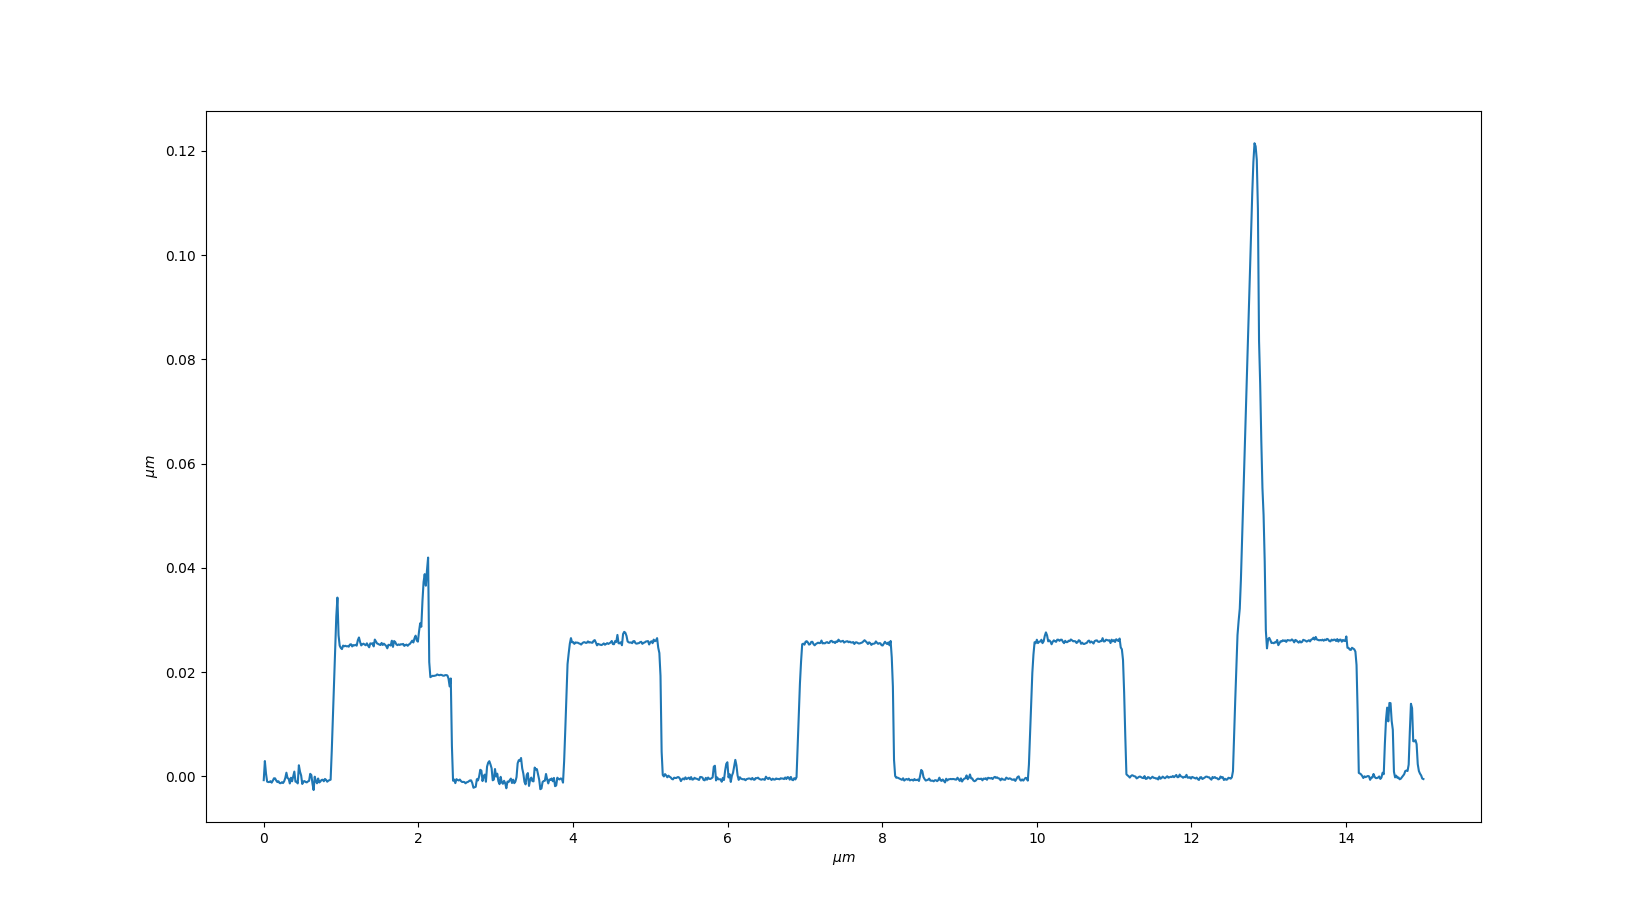
\includegraphics[width=0.75\textwidth]{../images/steps_1.png}
    \captionof{figure}{Starting profile with noise}
\end{center}
To detect the position, the height and the width of the steps we proceed in the following way:
\begin{itemize}
    \item Calculate the mean of the profile and we substract the average value of all the points laying below the mean value.
    \item Create the mask of the points that have an height between the nominal height and its $\sigma_{std}$.
\end{itemize}
\begin{center}
    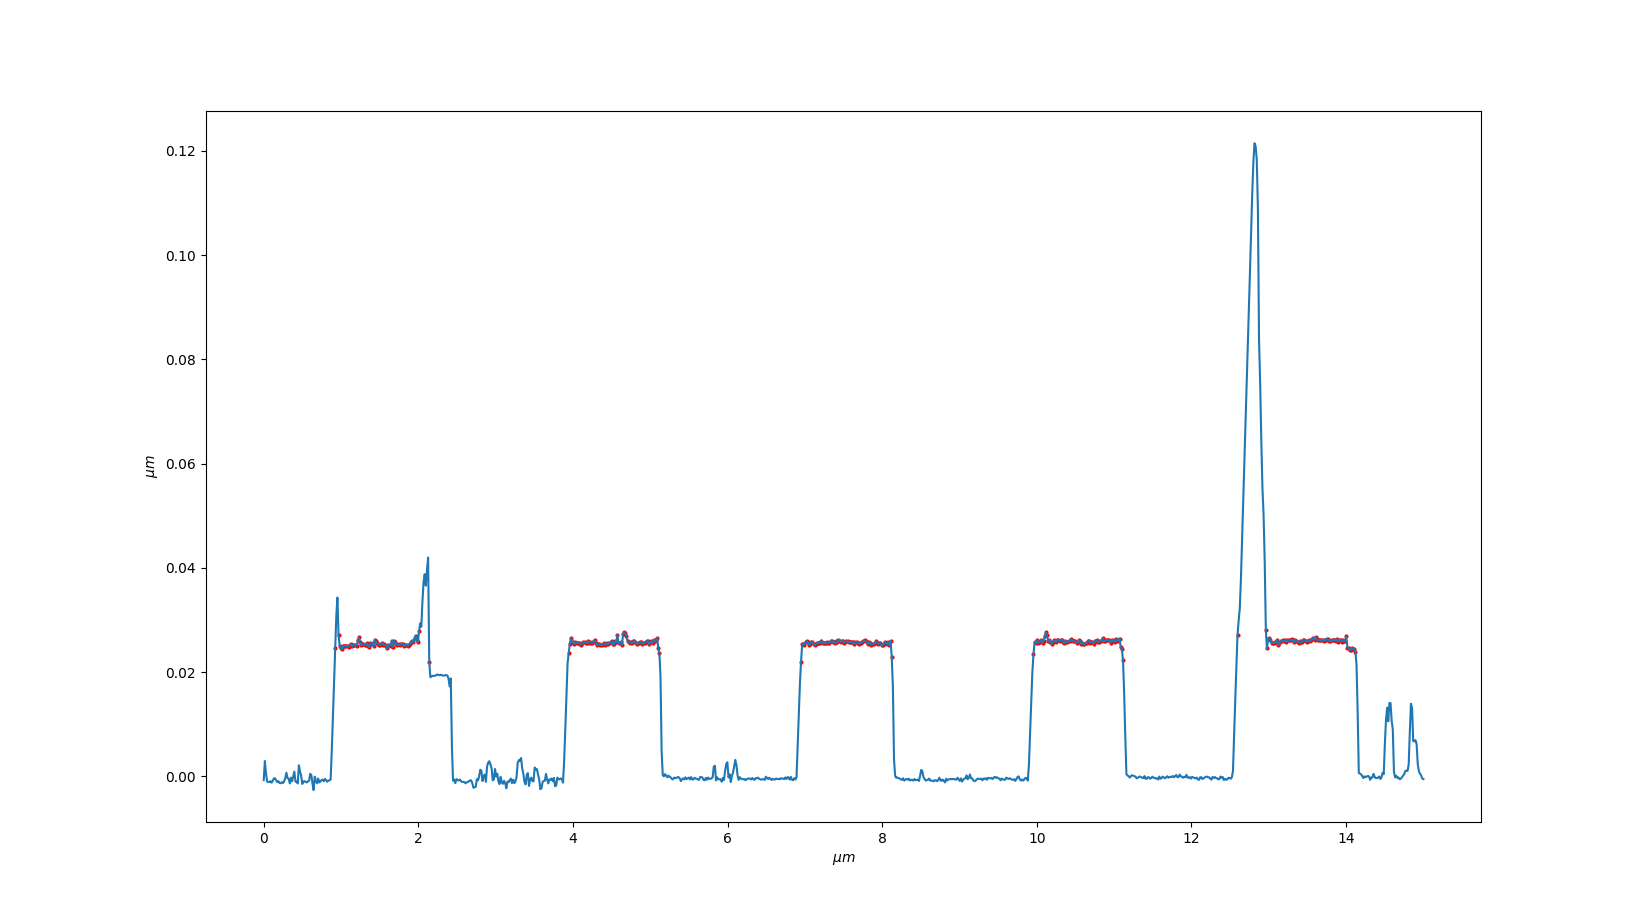
\includegraphics[width=0.75\textwidth]{../images/steps_2.png}
    \captionof{figure}{Choosing all the suitable points in the nominal height radius}
\end{center}
\begin{itemize}
    \item Calculate the derivative of this mask and find the indices of the points corresponding to raising and falling edges.
\end{itemize}    
\begin{center}
    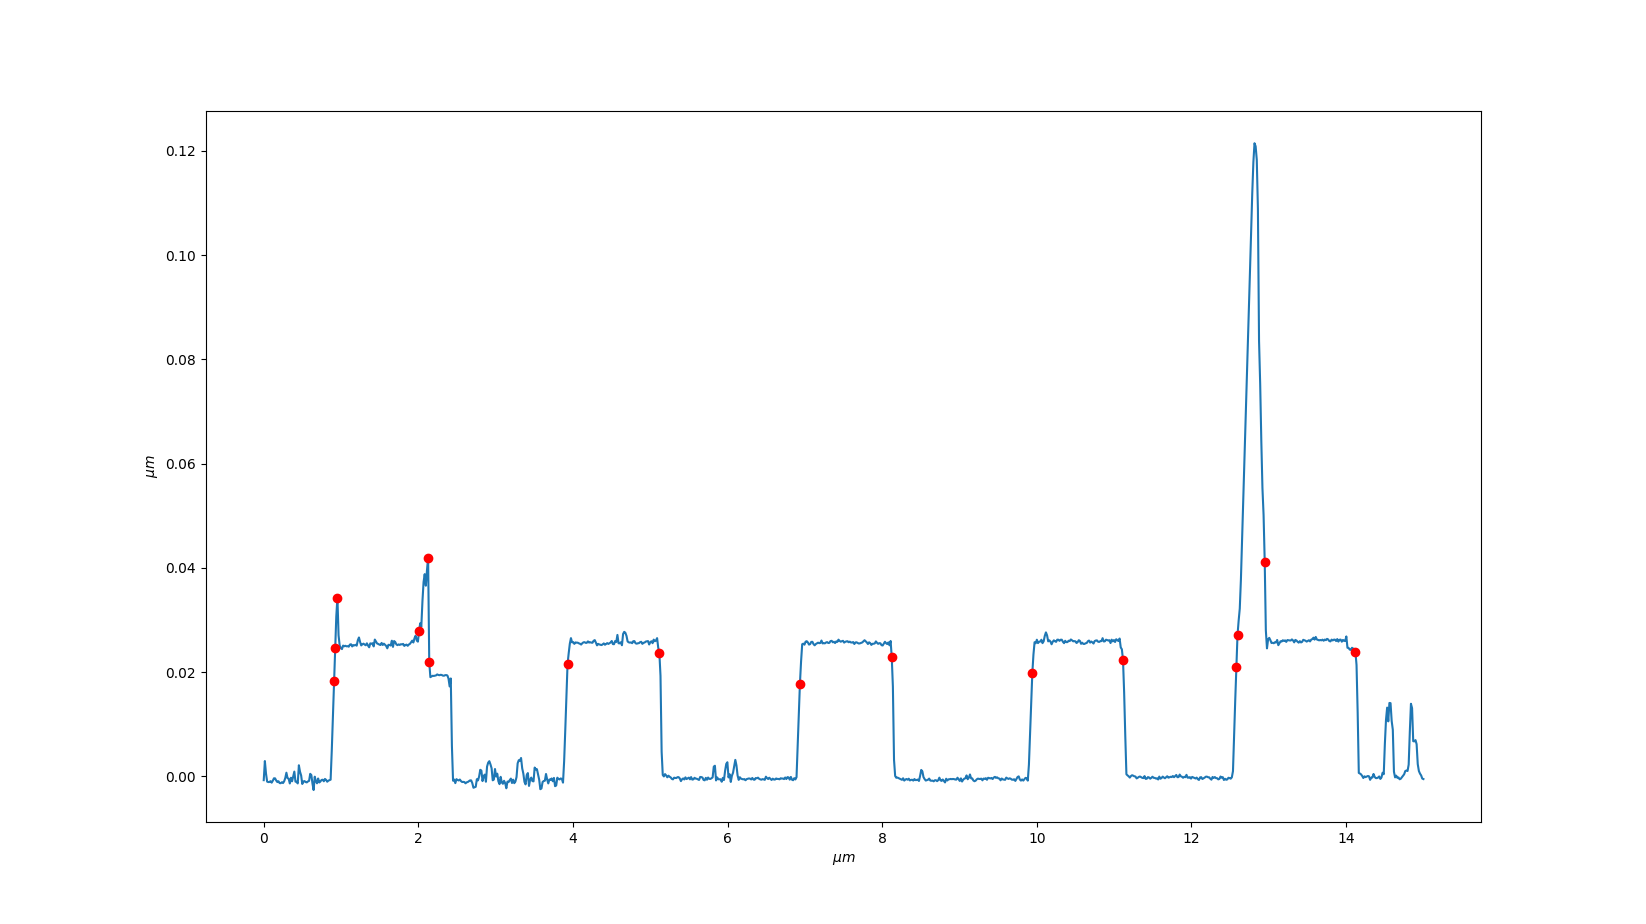
\includegraphics[width=0.75\textwidth]{../images/steps_3.png}
    \captionof{figure}{Finding all the derivative points}
\end{center}
\begin{itemize}
    \item Calculate width of the nominal step in pixels (from the nominal width in $\mu m$).
\end{itemize}
We then calculate the width of the measuered peak using the following algorithm:
\paragraph{Peak width and center detection algorithm: }

\begin{itemize}
    \item Initialize a \texttt{best\_width\_candidate} which will assume over time the best guess for the width of the step
    \item Take the first element of the derivative and consider it as the \texttt{start\_index}.
    \item Take the next element and consider it as the end of the step (\texttt{stop\_index}) 
    \item Check if the difference between the 2 indices is closer to the nominal width of the step than the best guess, if so update the \texttt{best\_width\_candidate}.
    \item Once the difference between the 2 considered values exceedes 1.5 of the nominal width, consider the next point as a new starting position
    \item At this point save the found values and update the reconstructed profile with the mean of each peak all the points that fall in the range of $h \pm \sigma_{h}$
    \item Repeat the process until all the elements have been processed.
\end{itemize}
\begin{center}
    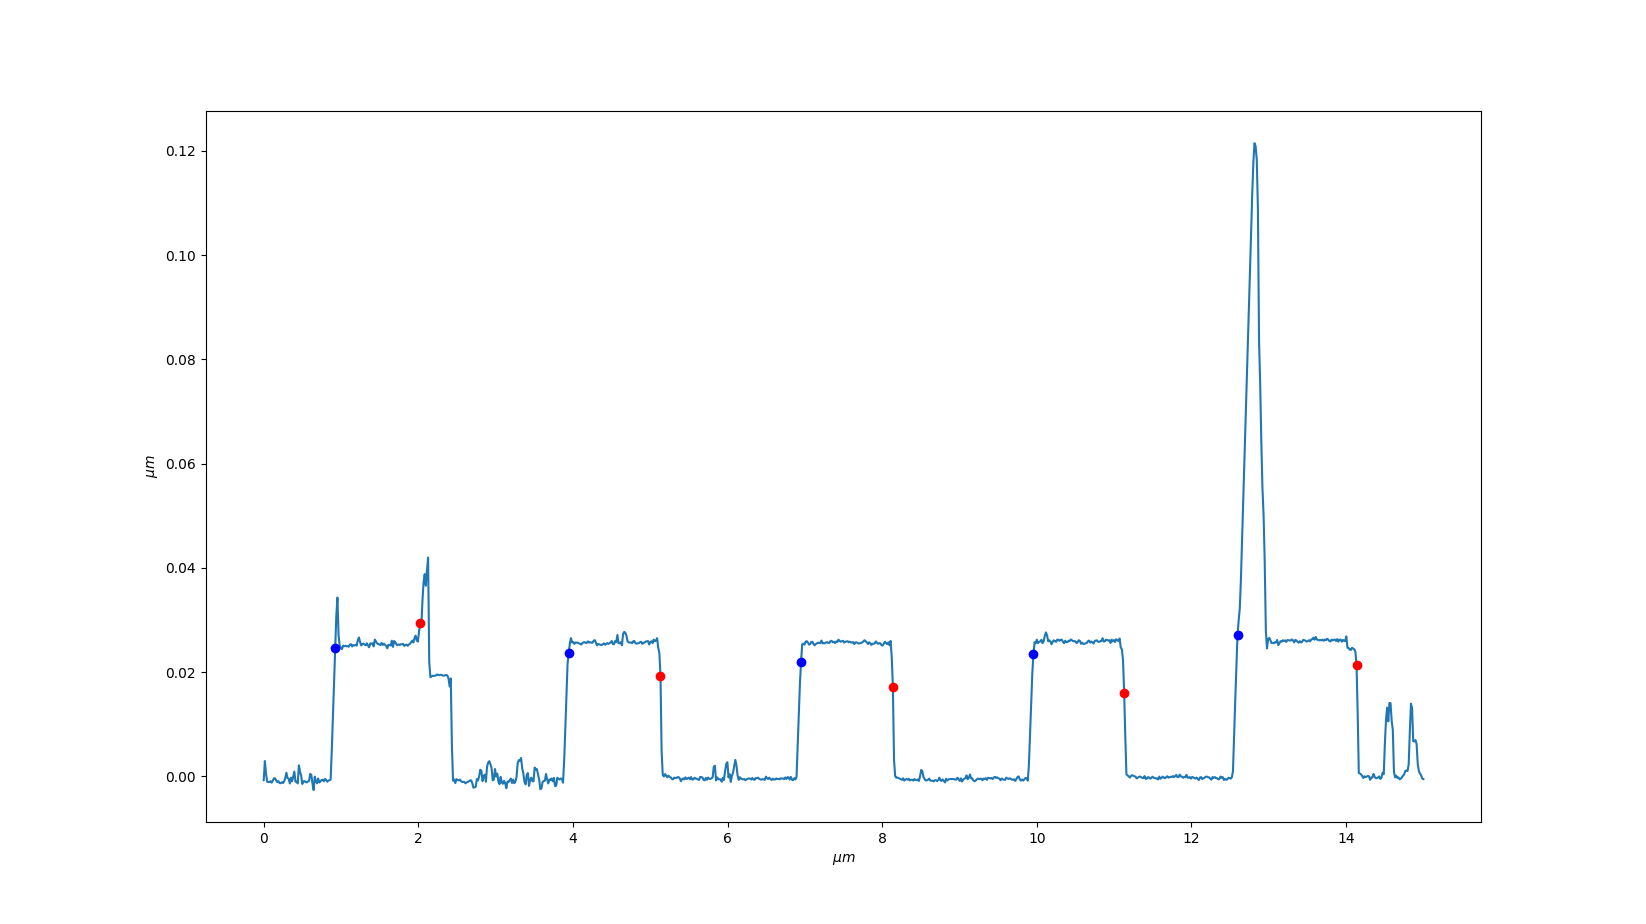
\includegraphics[width=0.75\textwidth]{../images/steps_4.png}
    \captionof{figure}{Choosing the best values based on the algorithm described in the next paragraph}
\end{center}

% \begin{center}
%     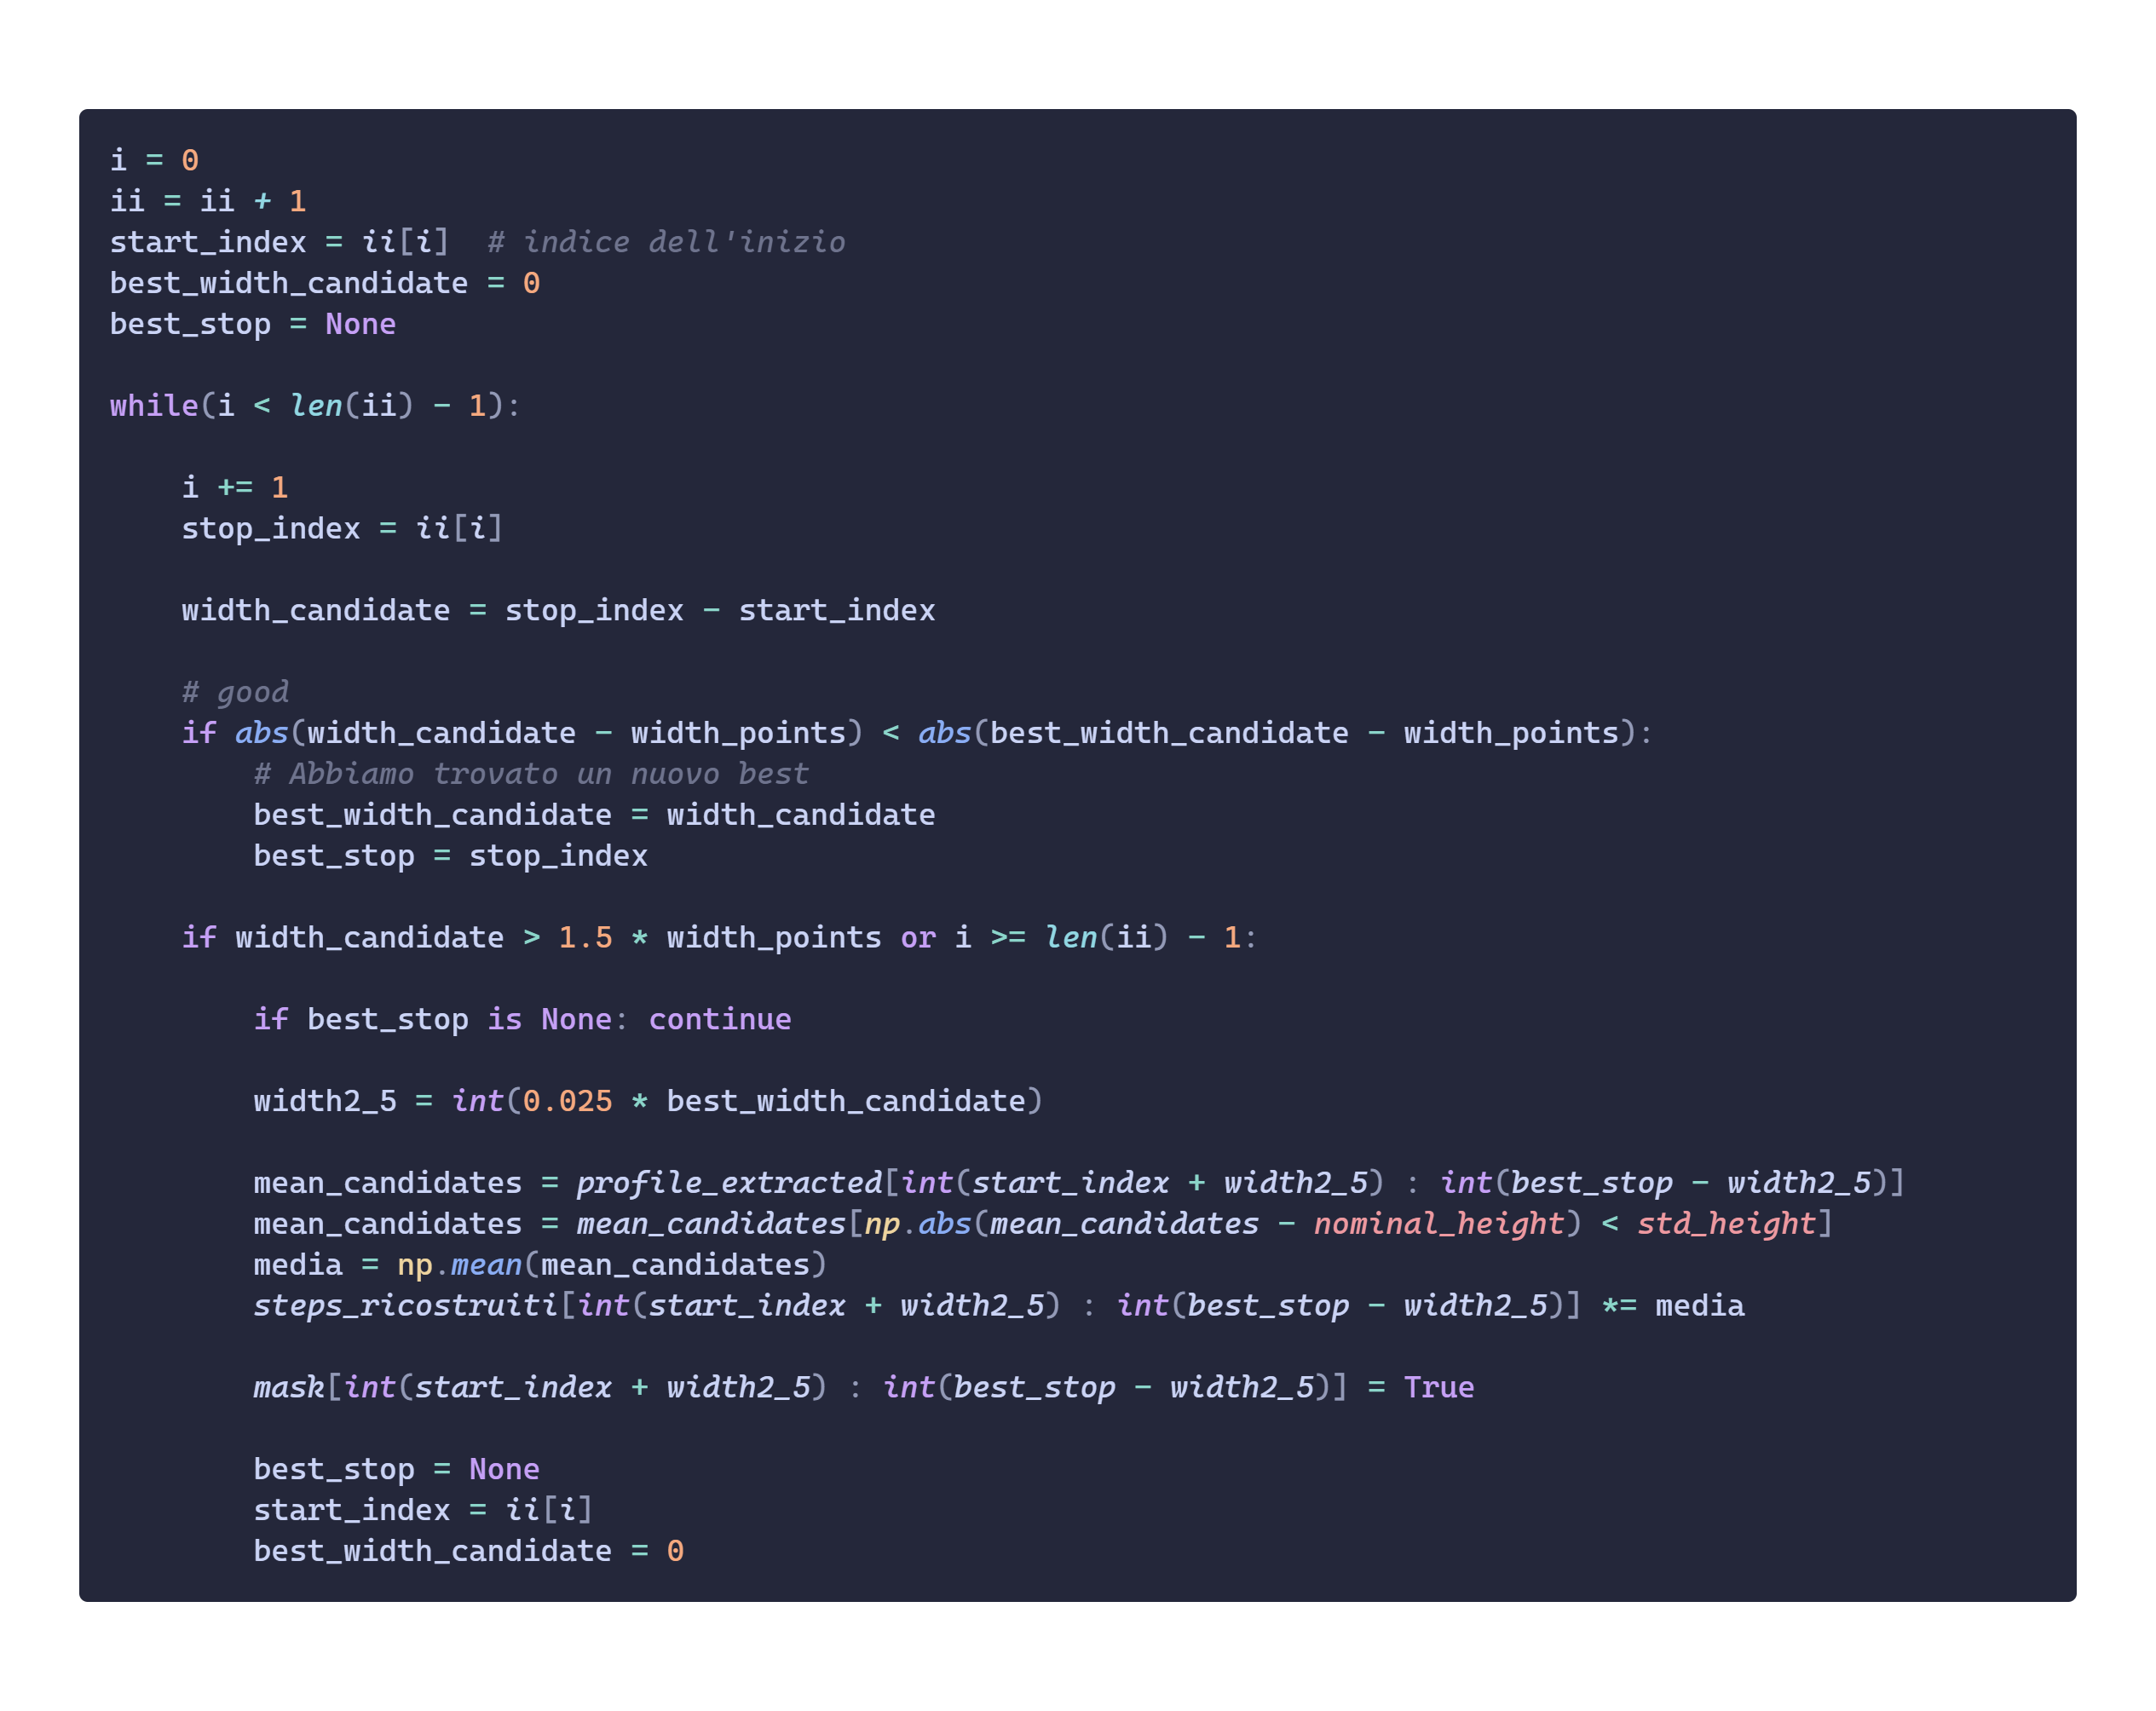
\includegraphics[width=\textwidth]{../images/while_code.png}
% \end{center}

\begin{center}
    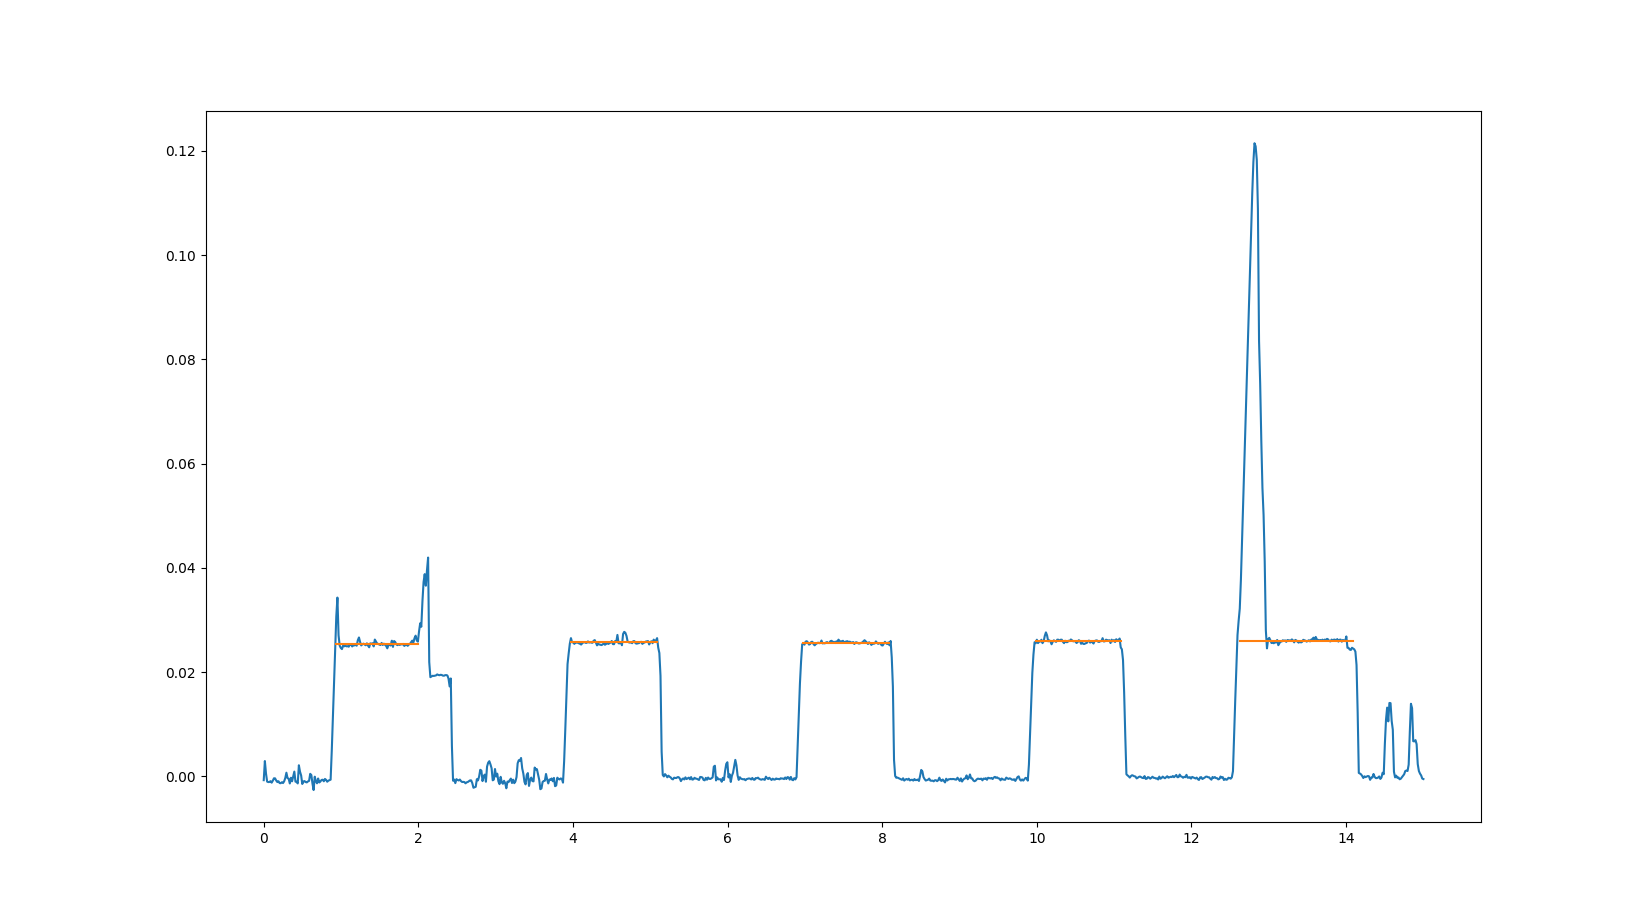
\includegraphics[width=0.75\textwidth]{../images/steps_5.png}
    \captionof{figure}{Generated structure based on the mean values}
\end{center}

\newpage

\section{Structure fitting}\label{sec:Structure_fitting}
\subsection{Sphere fitting}\label{subsec:Sphere_fitting}
This algorithm is implemented in \texttt{Recognizer.recognize\_sphere} and it is used to find the best position and parameters of an ideal sphere that needs to be fitted under the measured AFM data. To do so, the algorithm begins by finding the maximum peaks in the image data. This is done by using \texttt{scipy.maximum\_filter}:
\begin{center}
    \includegraphics[width=.5\textwidth]{../images/max_filter.png}
    \captionof{figure}{Mathematical rappresentation of the maximum filter}
    \label{fig:max_filter}
\end{center}

\begin{lstlisting}[style=Pythonstyle, caption={Implementation of the local maxima}]
local_max = maximum_filter(self.deconvoluted.Z, footprint=neighborhood)==self.deconvoluted.Z
local_max &= self.deconvoluted.Z > self.threshold
\end{lstlisting}

As shown in Fiugre \ref{fig:max_filter} this algorithm finds for each $n \times n$ the maximum value and replaces the center of the neighbourhood with this value. At the end of the substitutions, only the values that remained unchanged with respect to the original unfiltered data are considered as local maxima as shown in Figure \ref{fig:sphere_rec}b.
All the filtered values are then filtered again to obtain only the peaks corresponding to the center of the nanospheres. This can be done by discarding all the noise peaks that are below the nominal radius of the nanoparticle.

Once all the centers have been found, the radius value for each nanoparticle is calculated by evaluating the height map at the center positions of the peaks. This is possible since the error caused by the physical interaction between the tip and the sample is negligible when the contact vector is perpendicular to the surface. Thus the radius is half the height of the topography at the center point. 

\begin{center}
    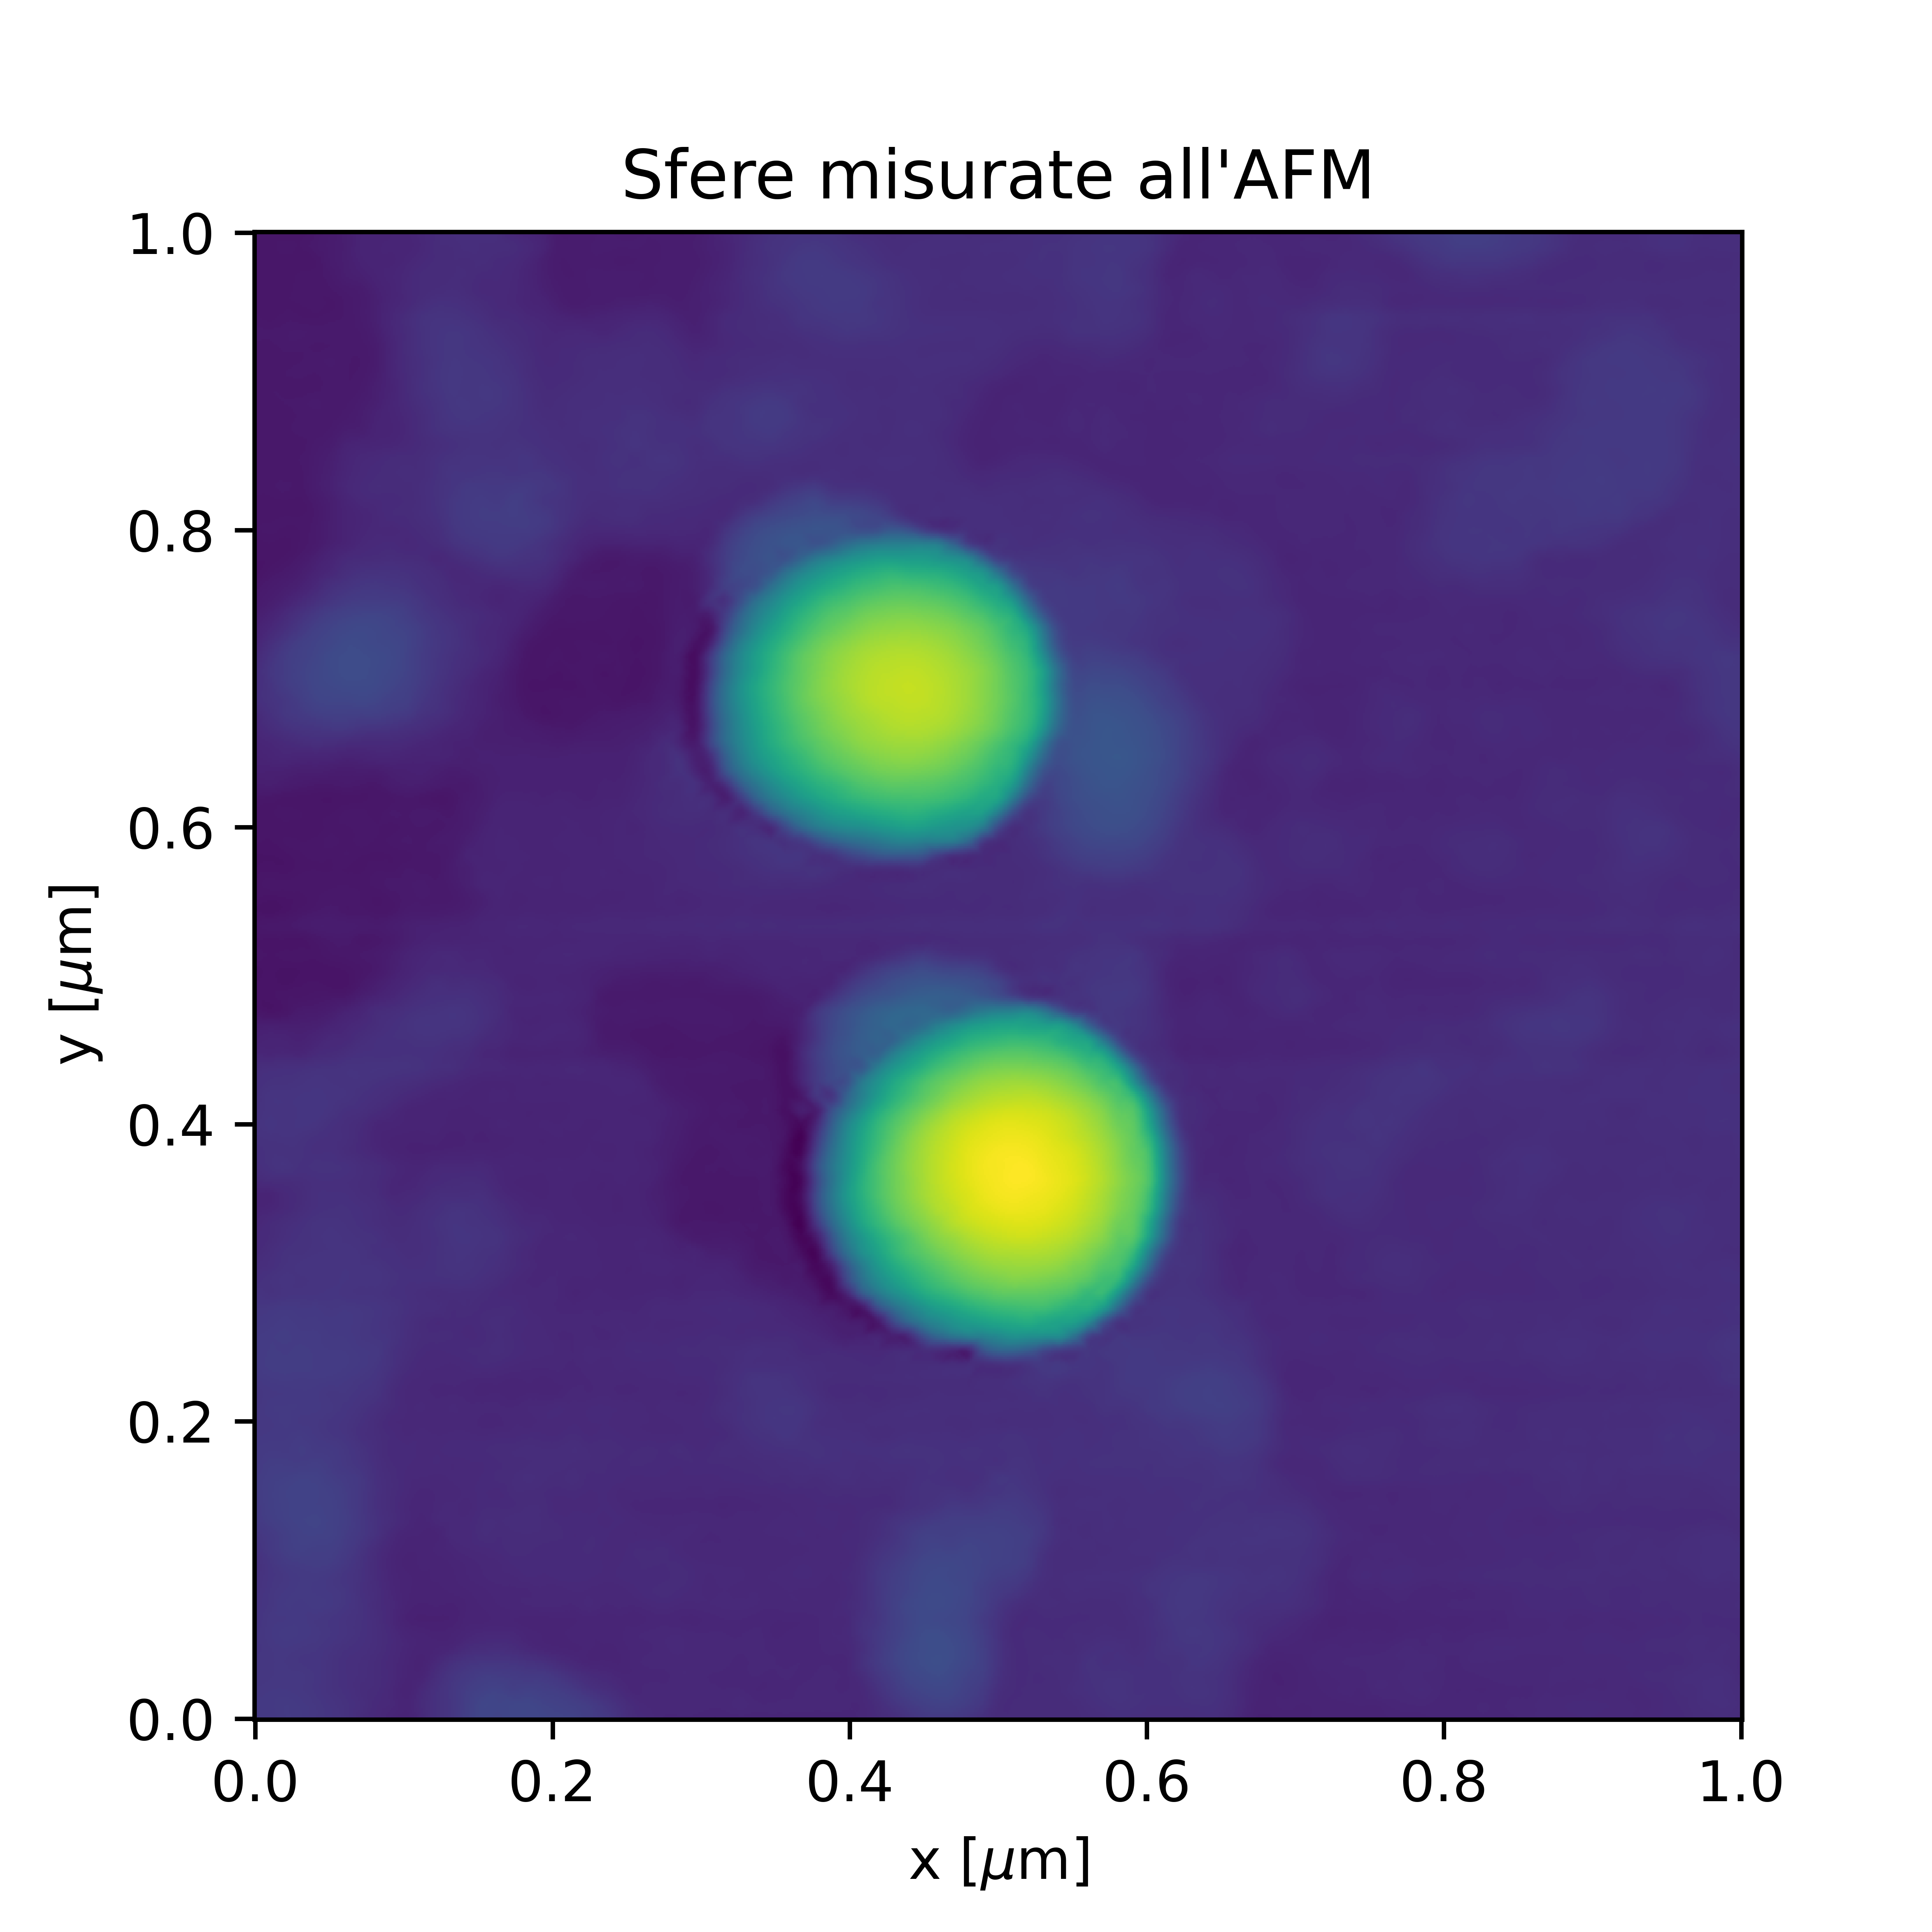
\includegraphics[width=.32\textwidth]{../images/original_data.png}
    \hfill
    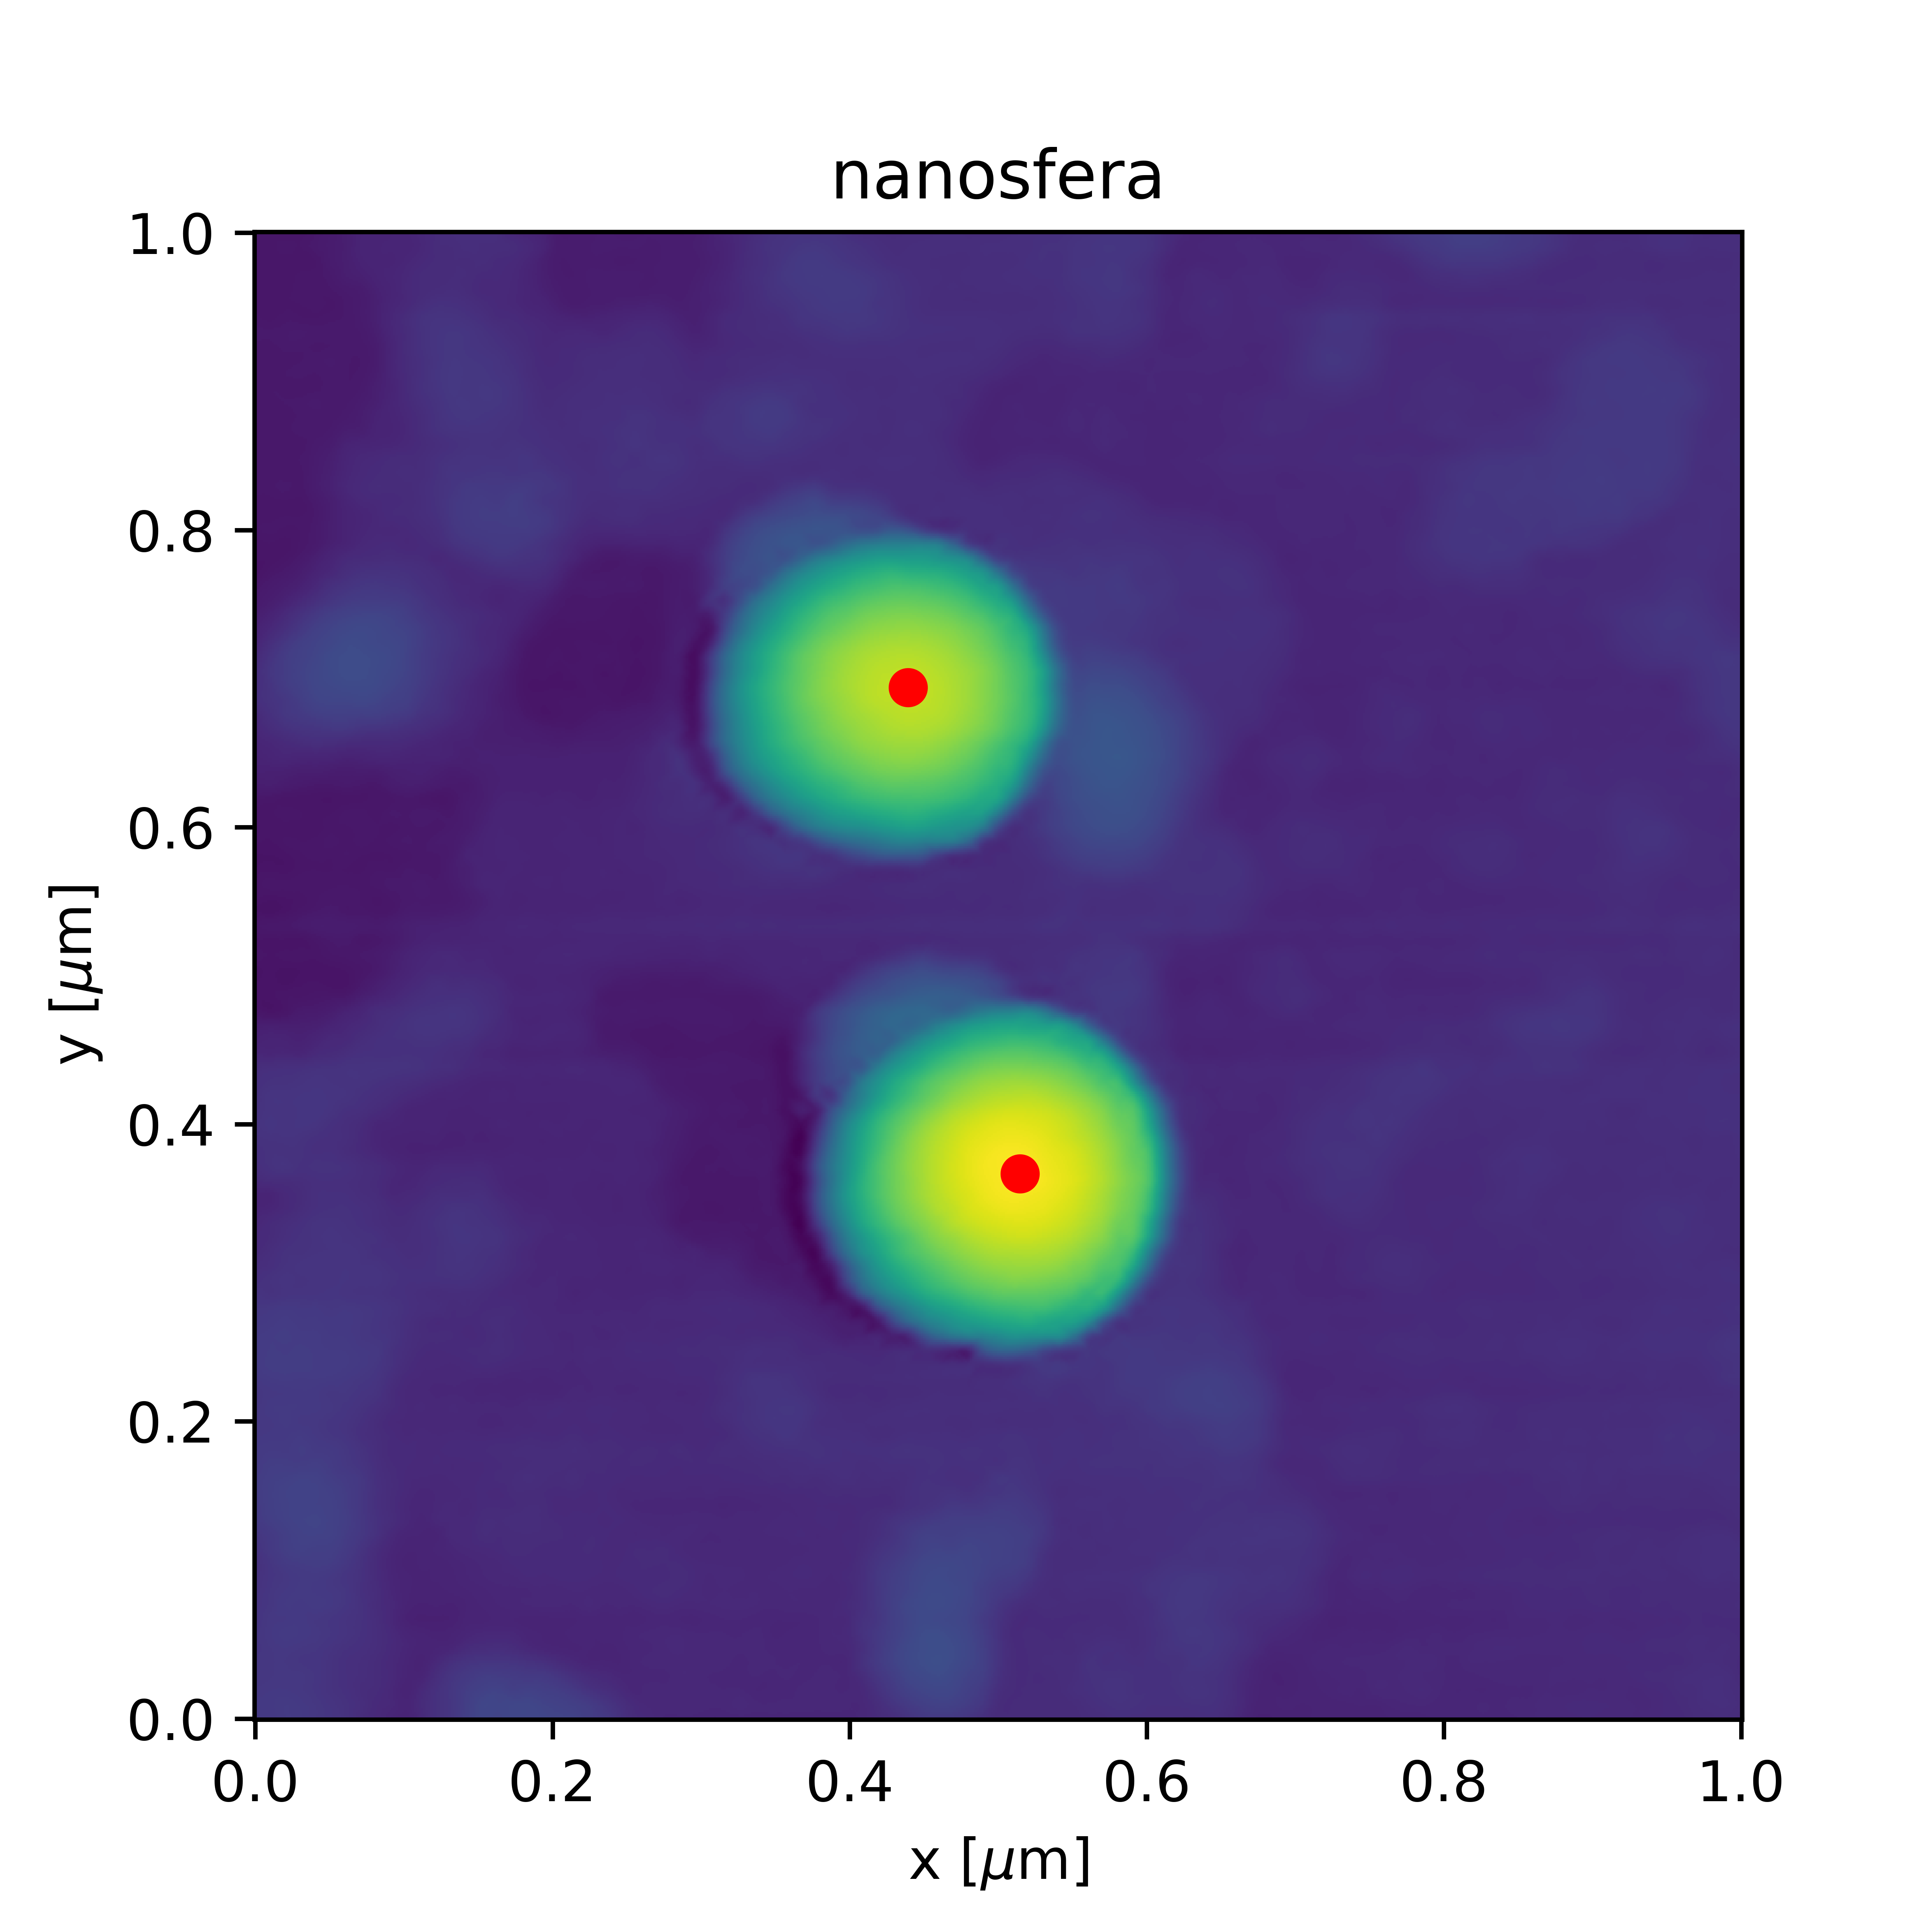
\includegraphics[width=.32\textwidth]{../images/found_peaks.png}
    \hfill
    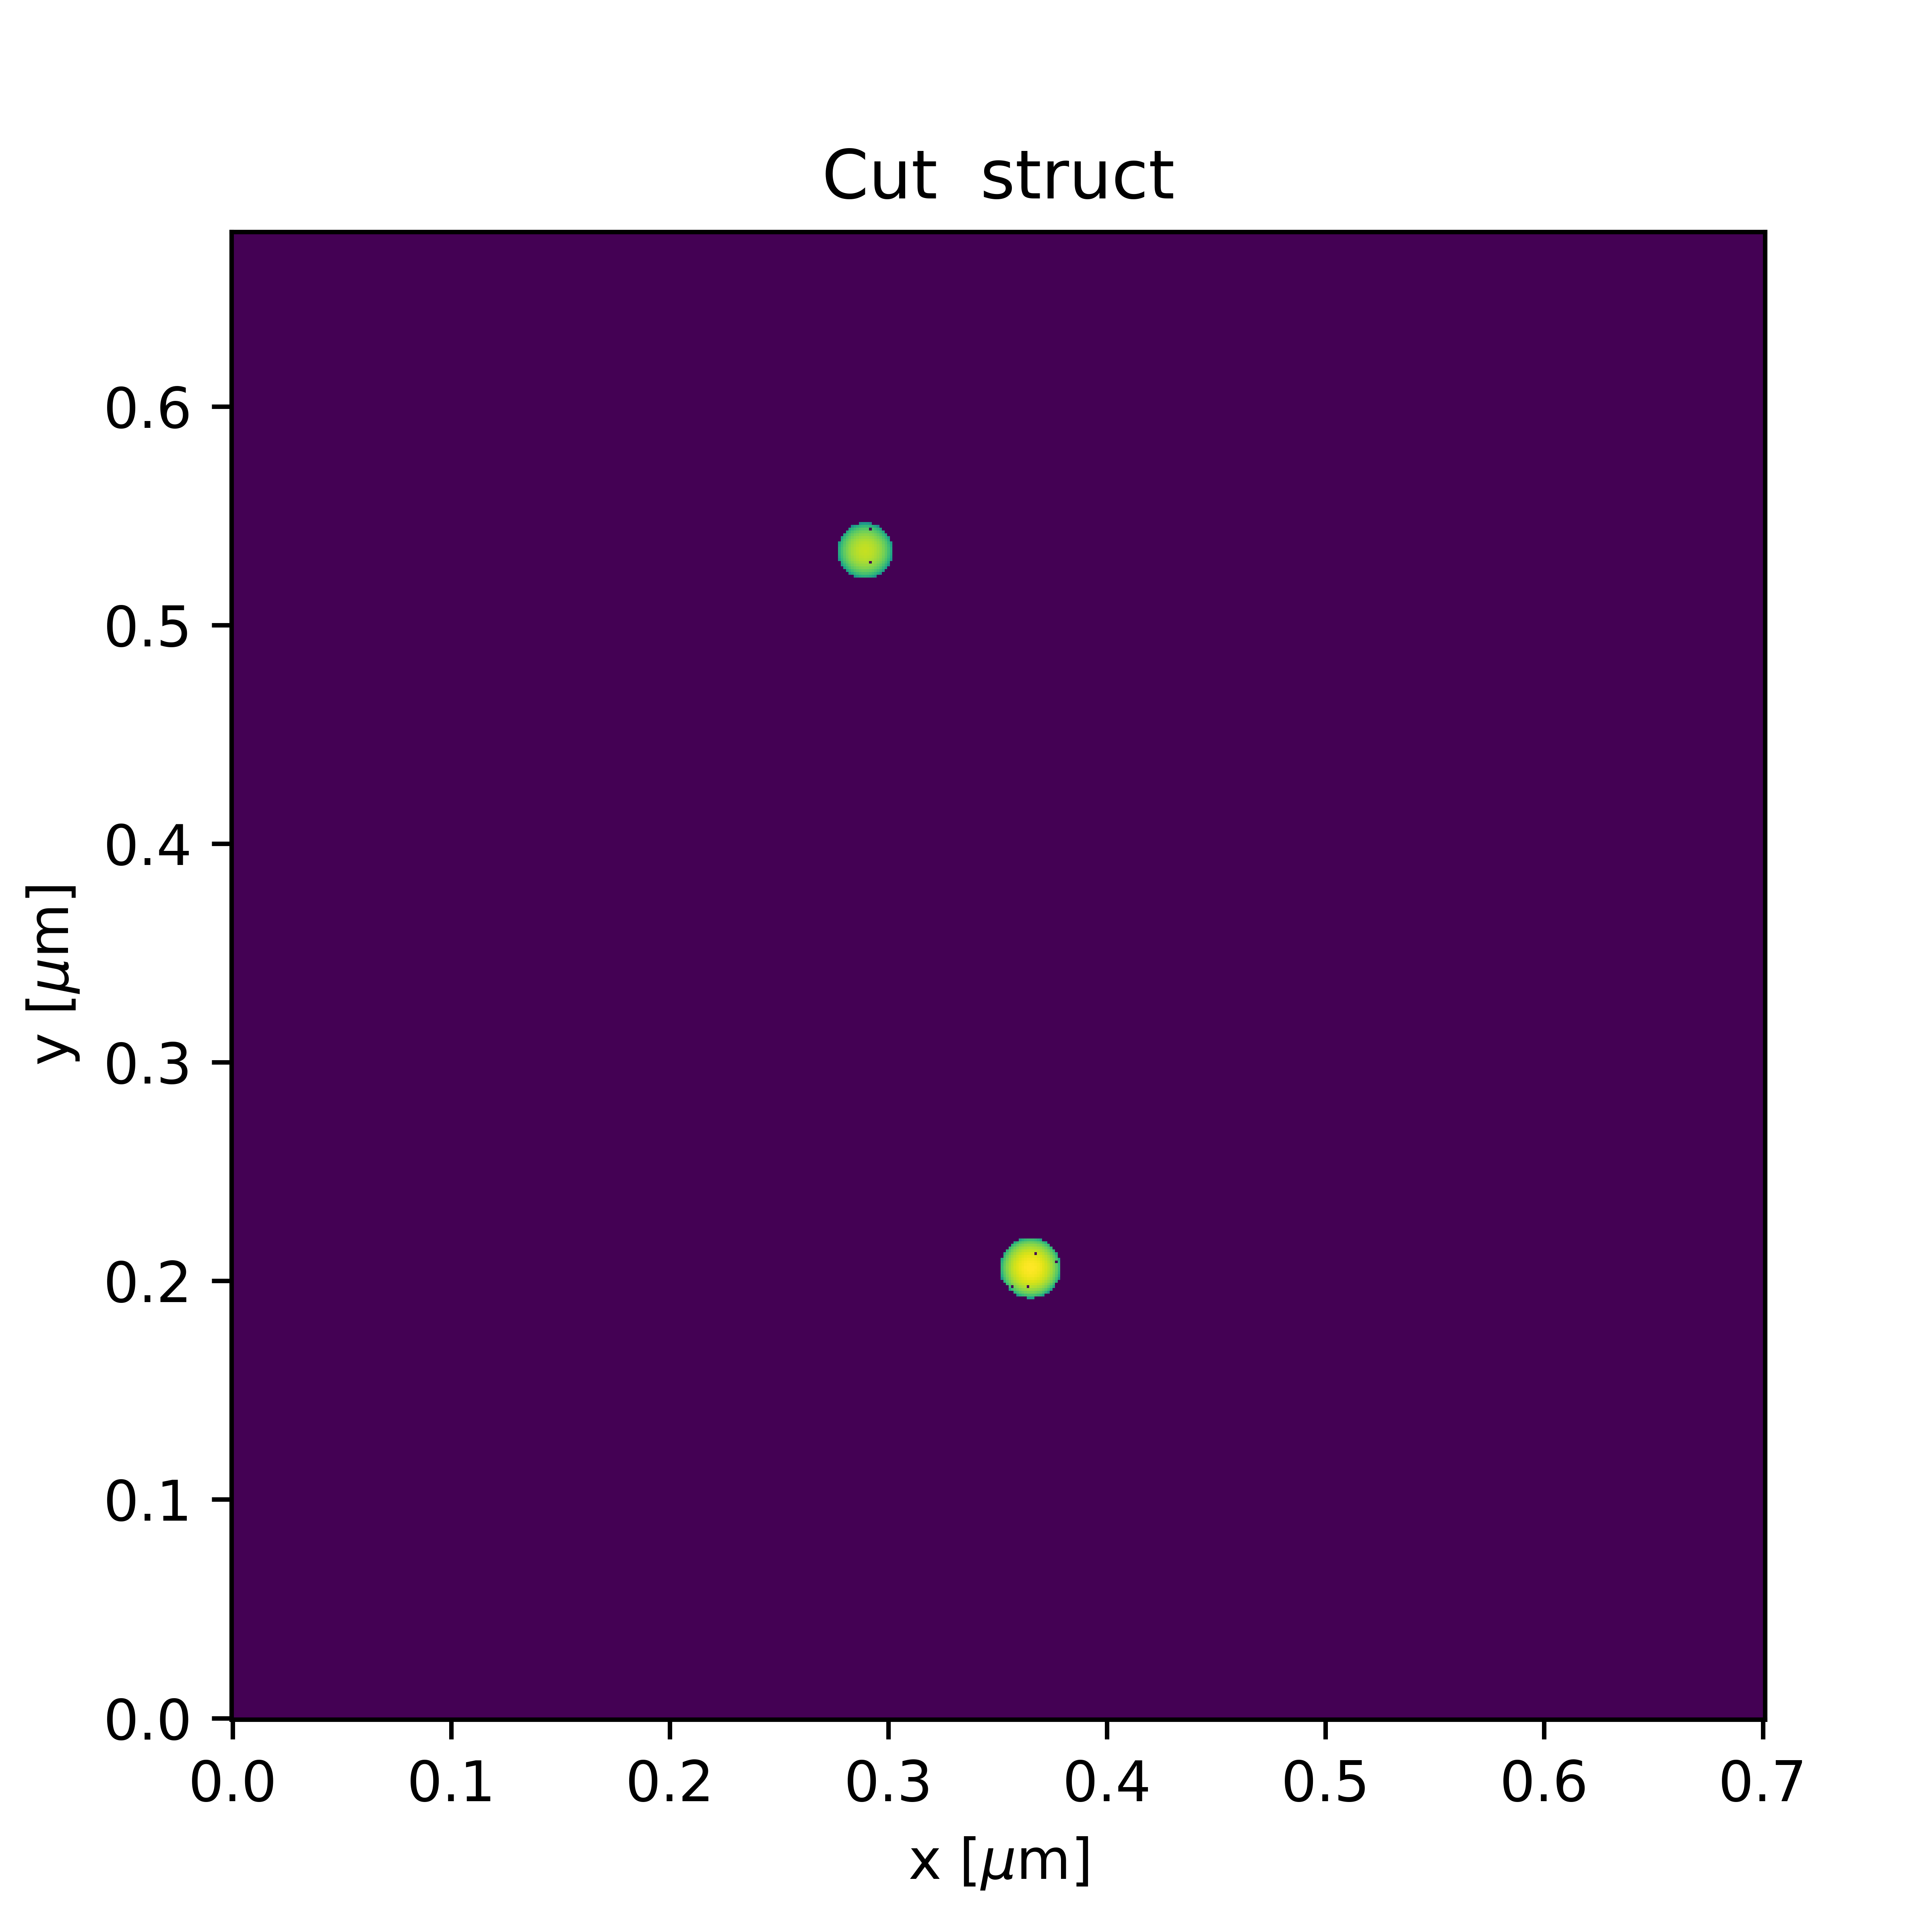
\includegraphics[width=.32\textwidth]{../images/ideal_structures.png}
    \captionof{figure}{a) Original data, b) Revealed peaks, c) Fitted ideal structures }
    \label{fig:sphere_rec}
\end{center}

\subsection{Tip size estimation}
Once the structures have been fitted under the topography, the tip matrix size must be estimated to cover the largest sample present in the image.
It is important though to not overestimate this parameter in order to have an high resolution tip after the erosion process. In fact, the size of the convolution output matrix is determined by the difference in the number of pixels between the structural size and the original data size.
Also underestimating the tip matrix size would be an issue, since the result would include only the tip apex resulting in the loss of tip sides.

To estimate the largest feature in the sample we approach the problem by creating a mask (Figure \ref{fig:mask}a) that selects only the points with the height value greater then a given treshold.
Then we calculate the derivative of this boolean mask along $X$ and $Y$ direction, obtaining the perimeter of this areas (Figure \ref{fig:mask}b).

\begin{center}
    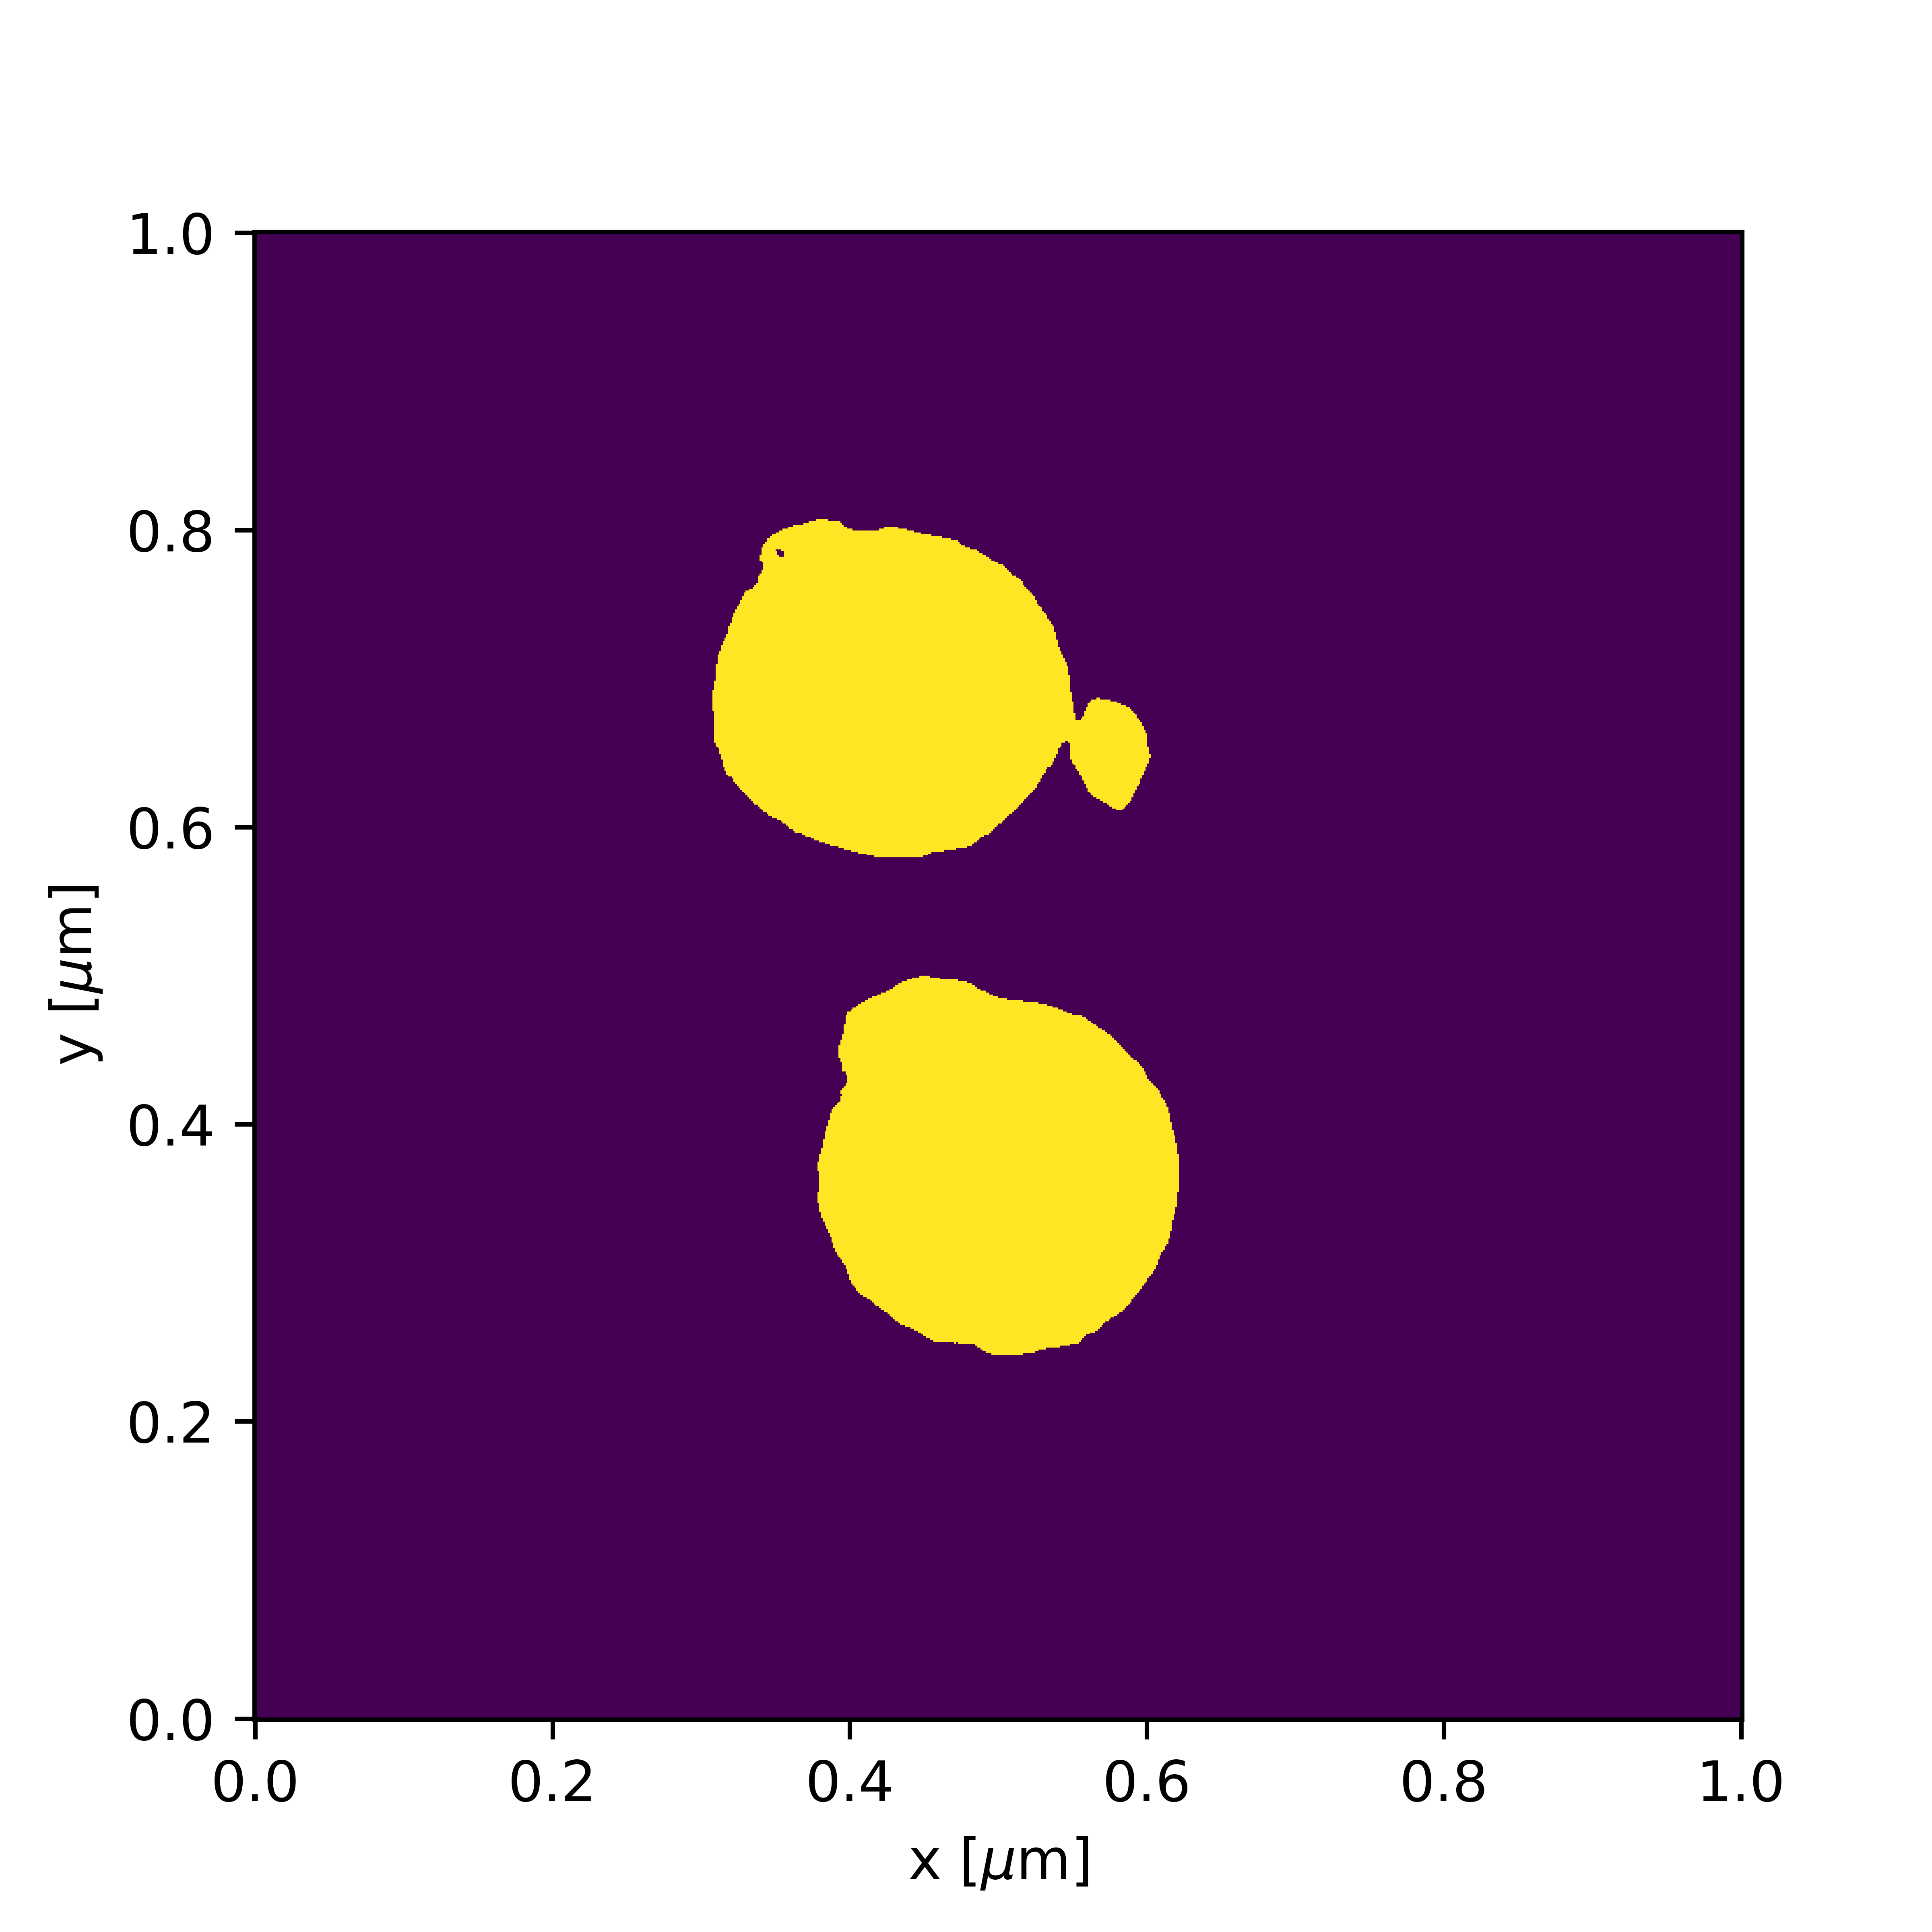
\includegraphics[width=.45\textwidth]{../images/maschera_picchi.png}
    \hfill
    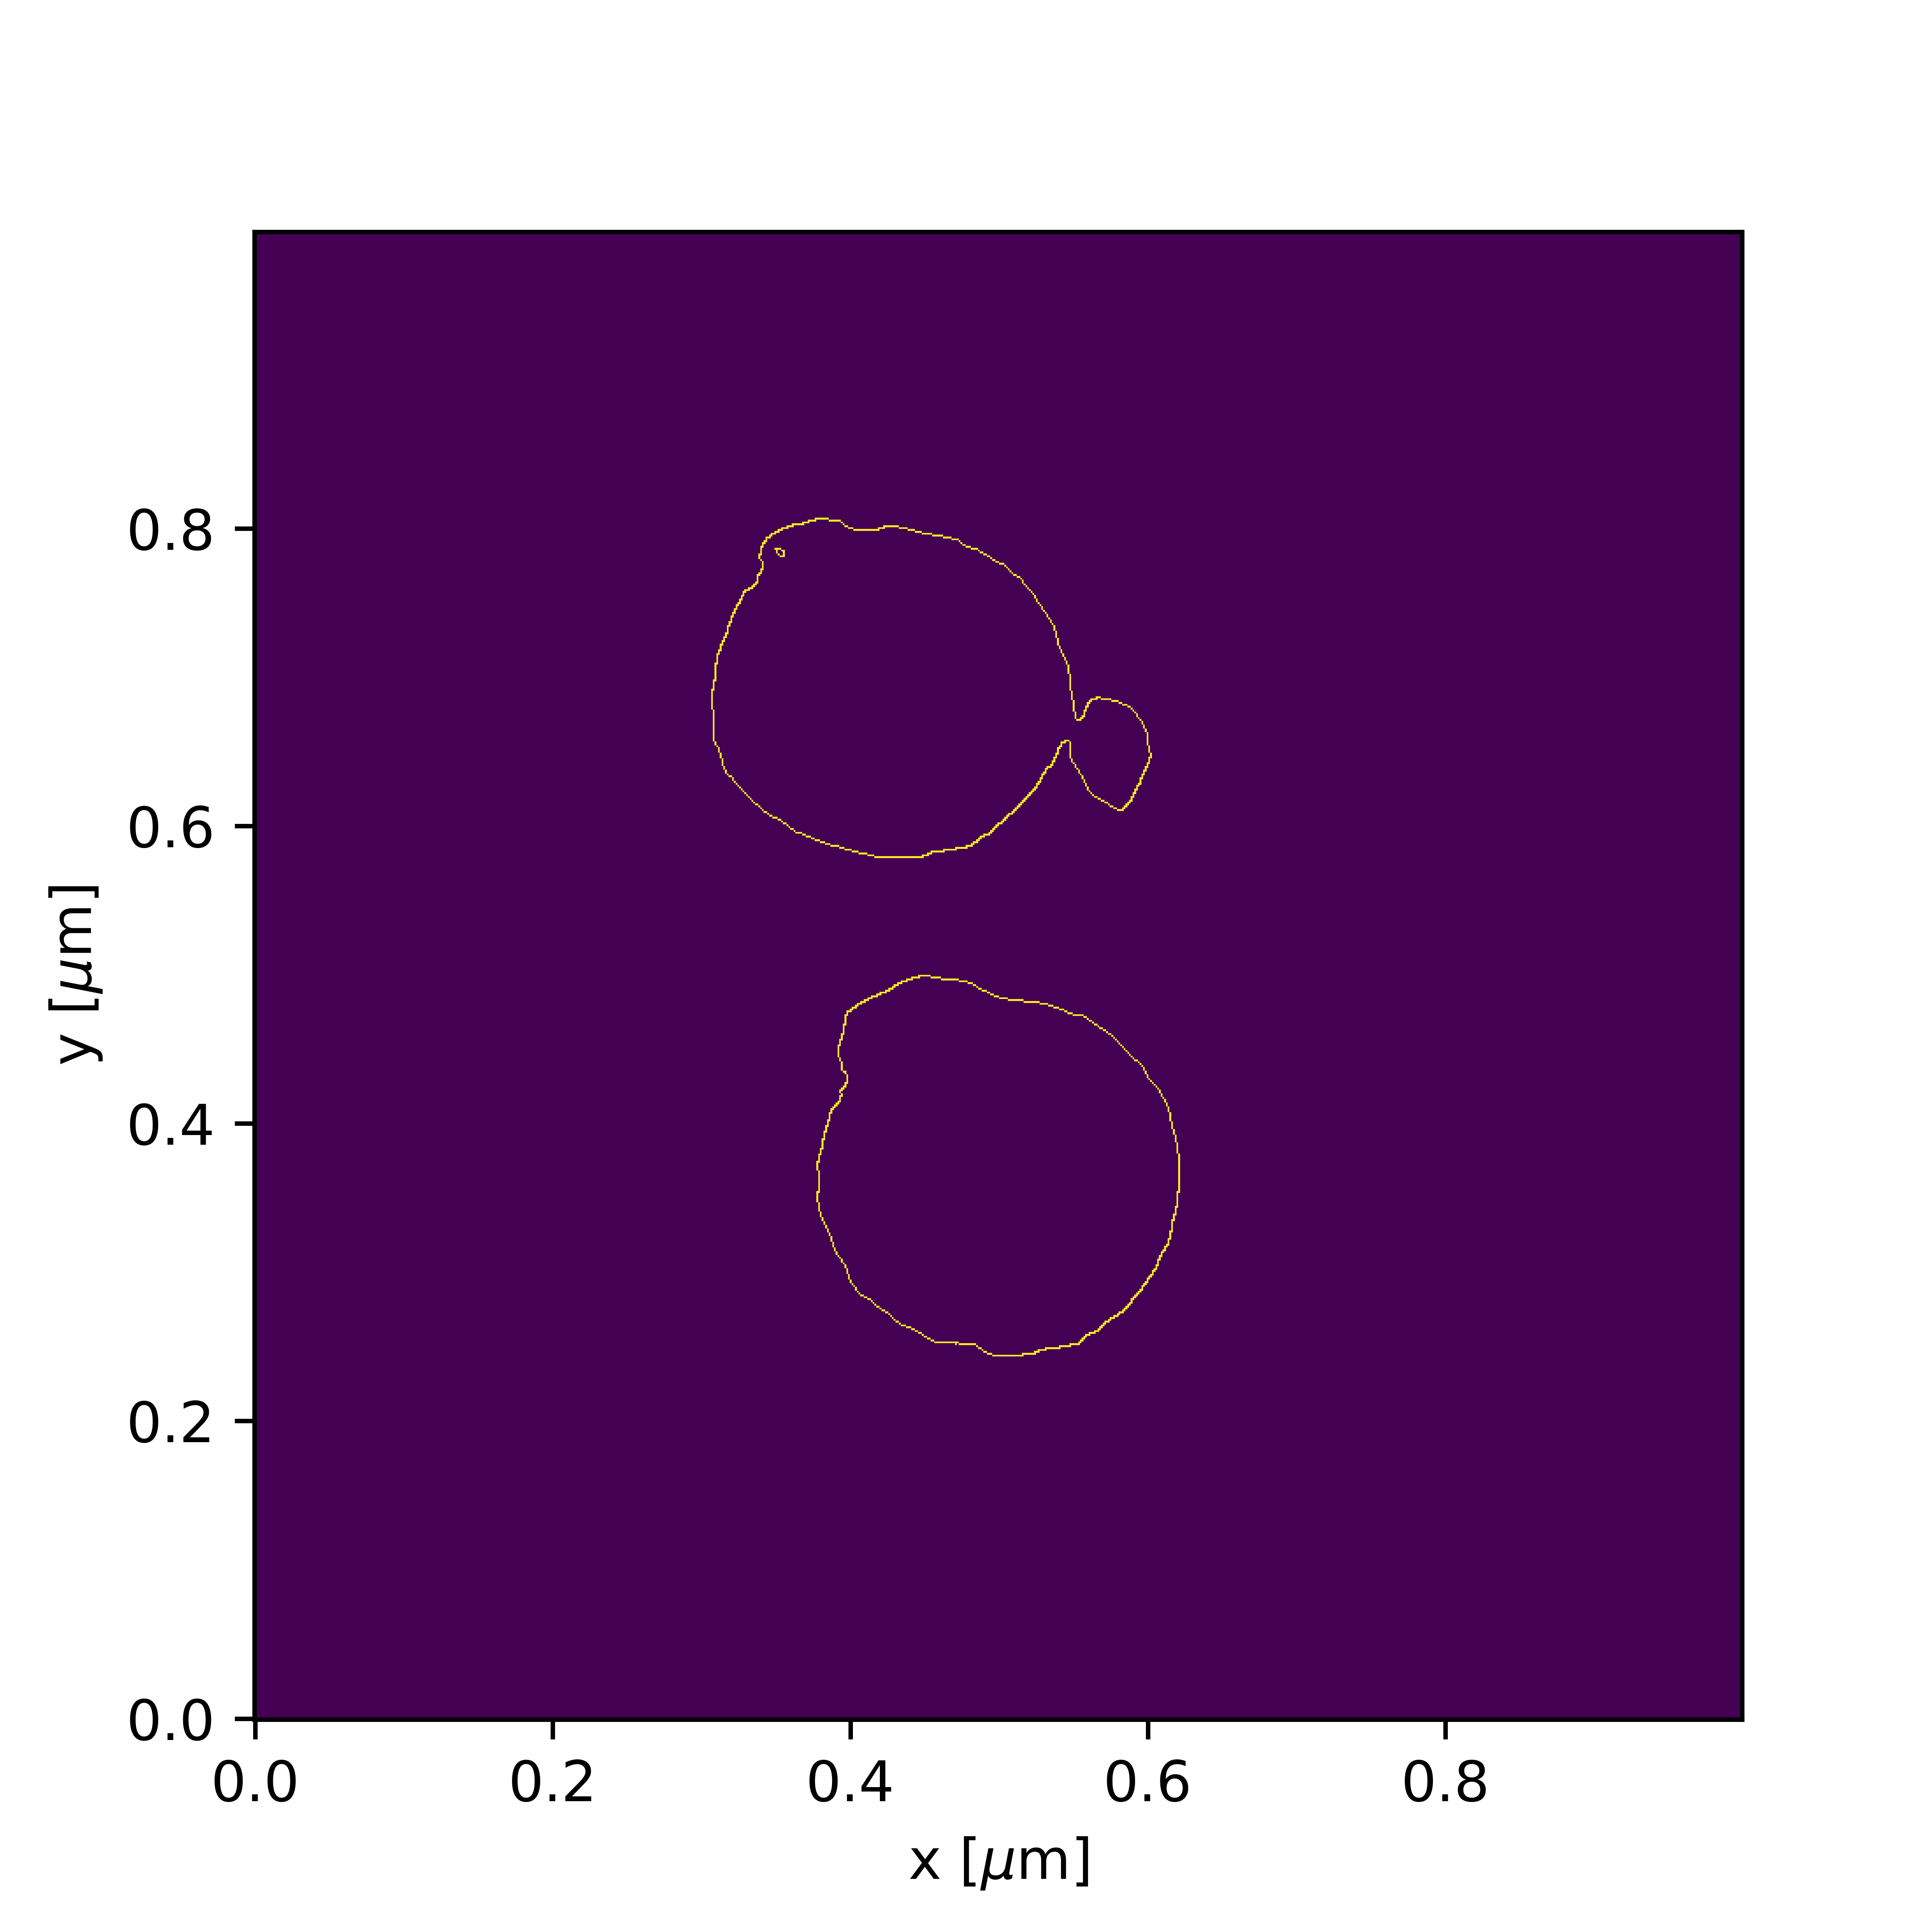
\includegraphics[width=.45\textwidth]{../images/derivatives.png}
    \captionof{figure}{a) Data mask of peaks vs background, b) Derivative of the mask in X and Y direction}
    \label{fig:mask}
\end{center}

This is beacuse the derivative of a boolean mask returns \texttt{True} if there's a change in the value of the data and \texttt{False} otherwise. We then scan line by line each in both directions and extracting all the \texttt{True} indices, we then couple them. The difference of the elements in each couple represents the width of the feature between the two indices. We finally take the maximum value of this difference and we use it as a parameter to obtain the final tip matrix size, which will be increased by an additional radius (example: $+10\%$) to guarantee a border around the reconstructed tip.   

\newpage

\section{Tip recounstruction}\label{sec:Tip_recounstruction}
\subsection{Erosion}\label{subsec:Erosion}

\begin{center}
    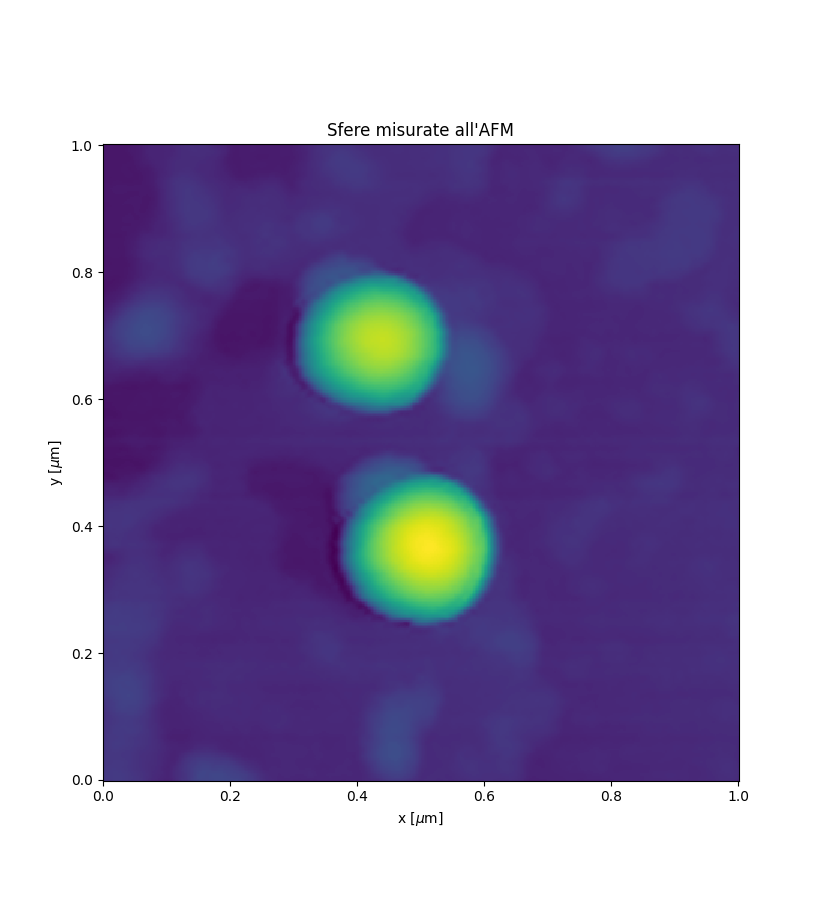
\includegraphics[width=.45\textwidth]{../images/deco_2d_1.png}
    \hfill
    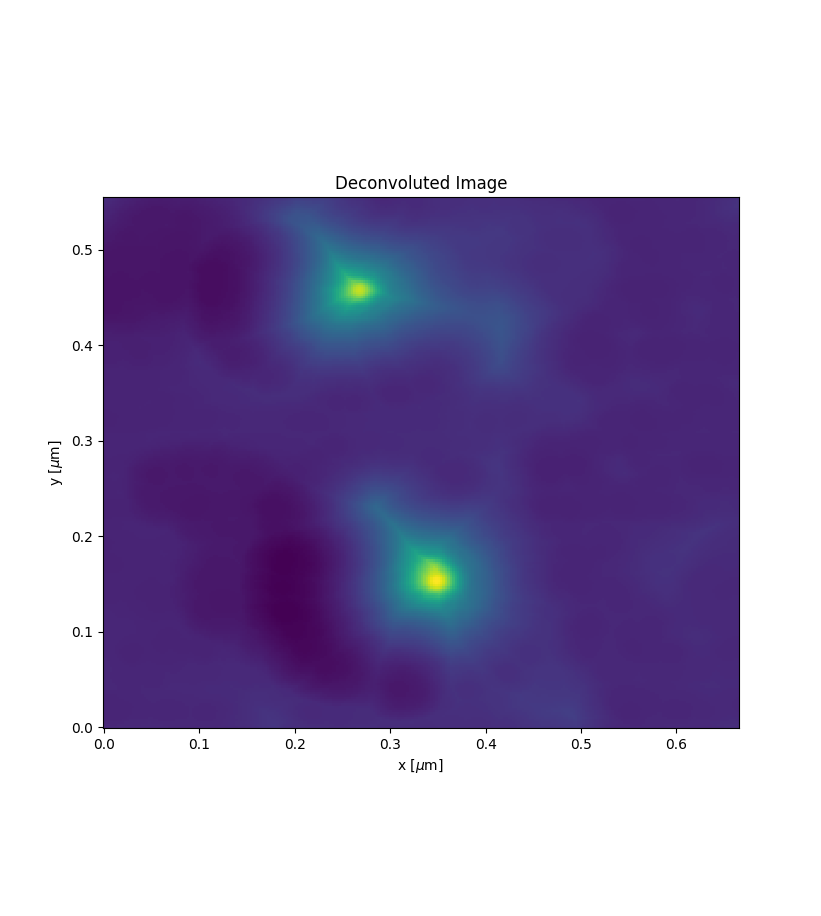
\includegraphics[width=.45\textwidth]{../images/deco_2d_2.png}
    \captionof{figure}{a) Original 2D AFM data b) Deconvoluted 2D AFM data}
    \label{fig:decon2d}
\end{center}

\begin{center}
    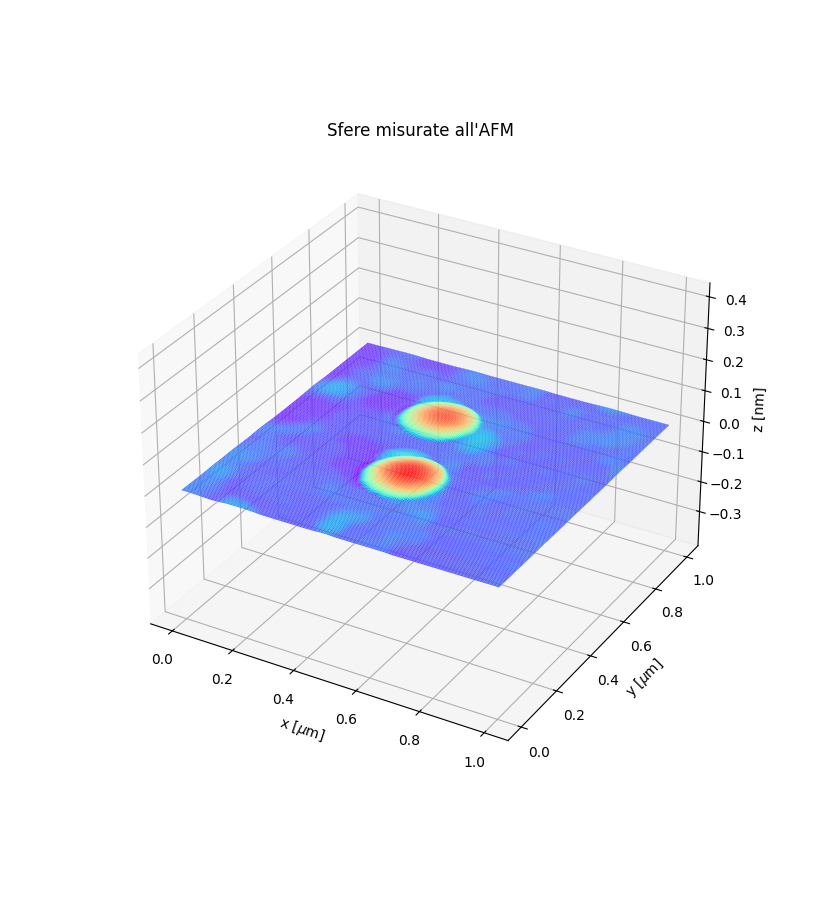
\includegraphics[width=.45\textwidth]{../images/deco_3d_1.png}
    \hfill
    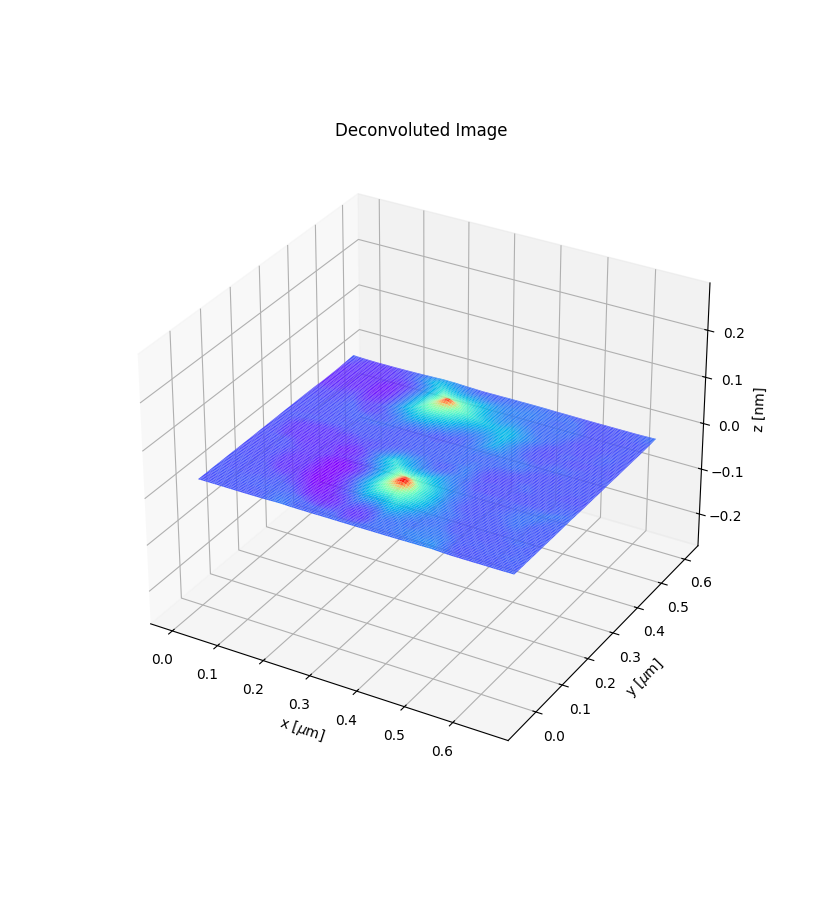
\includegraphics[width=.45\textwidth]{../images/deco_3d_2.png}
    \captionof{figure}{a) Original 3D AFM data, b) Deconvoluted 3D AFM data}
    \label{fig:decon3d}
\end{center}

\newpage

\section{References}
[1] G. B. Picotto, M. Vallino, L. Ribotta, Tip-sample characterization in the AFM study of a rod-shaped nanostructure, Meas. Sci. Technol., 31 (2020) 084001 (12 pp), DOI: 10.1088/1361-6501/ab7bc2
\\[.5cm]
[2] V. Maurino, F. Pellegrino, G. B. Picotto, L. Ribotta, Quantitative three-dimensional characterization of critical sizes of non-spherical TiO2 nanoparticles by using atomic force microscopy, Ultram. 234 (2022) 113480 (13 pp), DOI: 10.1016/j.ultramic.2022.113480
\\[.5cm]
[3] R. Bellotti, G. B. Picotto, L. Ribotta, AFM Measurements and Tip Characterization of Nanoparticles with Diferent Shapes, Nanomanufacturing and Metrology (2022) 5:127-138, DOI: 10.1007/s41871-022-00125-x
\\[.5cm]
[4] J. Villarrubia, Algorithms for scanned probe microscope image simulation, surface reconstruction, and tip estimation, J. Res. Natl. Inst. Stand. Technol 102 (4) (1997) 425-454. doi:10.6028/jres.102.030.


\end{document}
